\documentclass[11pt]{article}

% ACL submission style (review mode: anonymised, line numbers).
% Build with -jobname=main_camera "\def\CAMERAREADY{}\documentclass[11pt]{article}

% ACL submission style (review mode: anonymised, line numbers).
% Build with -jobname=main_camera "\def\CAMERAREADY{}\documentclass[11pt]{article}

% ACL submission style (review mode: anonymised, line numbers).
% Build with -jobname=main_camera "\def\CAMERAREADY{}\documentclass[11pt]{article}

% ACL submission style (review mode: anonymised, line numbers).
% Build with -jobname=main_camera "\def\CAMERAREADY{}\input{main.tex}"
% to obtain the camera-ready layout used by aclpubcheck.
\newif\ifaclreview
\aclreviewtrue
\ifdefined\CAMERAREADY\aclreviewfalse\fi
\ifaclreview\usepackage[review]{acl}\else\usepackage[final]{acl}\fi

\usepackage{times}
\usepackage{latexsym}
\usepackage[T1]{fontenc}
\usepackage[utf8]{inputenc}
\usepackage{microtype}
\usepackage{inconsolata}
\usepackage{graphicx}
\usepackage{capt-of}
\usepackage{booktabs}
\usepackage{amsmath}
\usepackage{amssymb}
\usepackage{xcolor}
\usepackage{tikz}
\usetikzlibrary{arrows.meta,positioning}
\usepackage{url}

\setlength{\tabcolsep}{4pt}
\setlength{\textfloatsep}{8pt plus 2pt minus 2pt}
\setlength{\floatsep}{6pt plus 2pt minus 2pt}
\setlength{\intextsep}{6pt plus 2pt minus 2pt}

\newcommand{\noul}{\textsc{Noul}}
\newcommand{\choice}{\textsc{Choice}}
\newcommand{\score}{\textsc{Score}}
\newcommand{\spanact}{\textsc{Span}}
\newcommand{\setact}{\textsc{Set}}
\newcommand{\eg}{e.g.,}
\newcommand{\ie}{i.e.,}

\title{When Evolutionary Routing Fails:\\ Action Complementarity and Utility Prediction in Structured Decision Models}

\author{Anonymous ACL submission}

\begin{document}
\maketitle

\begin{abstract}
Structured decision models such as Jev turn a language-model call into a typed
probabilistic judgment: a binary \noul{} decision, a candidate \choice{}, or a
\score{}. This interface makes inference-time routing attractive: ask a cheap
\noul{} question first and buy a second, differently framed \choice{} view only
when the first answer looks uncertain. We test that intuition with frozen open
models. Using Laya 0.4.16 and Vela 2.0 0.3B on CodeXGLUE defect detection,
FinDVer claim verification and ProcessBench reasoning-error localisation, we
compare a genetic algorithm, an evolution strategy and NSGA-II with fixed
policies and budget-matched random search, and measure per-example action
complementarity and the predictability of the second action's signed
incremental utility. Gross repair opportunities exist: a per-row oracle gains
up to 23.3 accuracy points over the better fixed action. Net repair is sparse
and pool-dependent: only one of four confirm cells has a positive accuracy
interval, and its macro-F1 interval still spans zero. Out-of-fold rank
correlation for a signed-utility predictor is weak ($|\text{Spearman}|\le
0.19$; every group-bootstrap interval includes zero), and confirm cost-adjusted
utility is non-positive in all four cells. No genetic-algorithm genome beats
the better fixed action, including on a one-shot locked test; the only
locked-test gain is over the worse fixed switch, where it learns to stay on
\noul{}. Calibration improves probabilities but does not create routing signal,
because monotone recalibration leaves the band policy class unchanged.
\end{abstract}

\input{sec_intro}
\input{sec_related}
\input{sec_method}
\input{sec_design}
\input{sec_results}
\input{sec_conclusion}

\bibliography{references}

\end{document}
"
% to obtain the camera-ready layout used by aclpubcheck.
\newif\ifaclreview
\aclreviewtrue
\ifdefined\CAMERAREADY\aclreviewfalse\fi
\ifaclreview\usepackage[review]{acl}\else\usepackage[final]{acl}\fi

\usepackage{times}
\usepackage{latexsym}
\usepackage[T1]{fontenc}
\usepackage[utf8]{inputenc}
\usepackage{microtype}
\usepackage{inconsolata}
\usepackage{graphicx}
\usepackage{capt-of}
\usepackage{booktabs}
\usepackage{amsmath}
\usepackage{amssymb}
\usepackage{xcolor}
\usepackage{tikz}
\usetikzlibrary{arrows.meta,positioning}
\usepackage{url}

\setlength{\tabcolsep}{4pt}
\setlength{\textfloatsep}{8pt plus 2pt minus 2pt}
\setlength{\floatsep}{6pt plus 2pt minus 2pt}
\setlength{\intextsep}{6pt plus 2pt minus 2pt}

\newcommand{\noul}{\textsc{Noul}}
\newcommand{\choice}{\textsc{Choice}}
\newcommand{\score}{\textsc{Score}}
\newcommand{\spanact}{\textsc{Span}}
\newcommand{\setact}{\textsc{Set}}
\newcommand{\eg}{e.g.,}
\newcommand{\ie}{i.e.,}

\title{When Evolutionary Routing Fails:\\ Action Complementarity and Utility Prediction in Structured Decision Models}

\author{Anonymous ACL submission}

\begin{document}
\maketitle

\begin{abstract}
Structured decision models such as Jev turn a language-model call into a typed
probabilistic judgment: a binary \noul{} decision, a candidate \choice{}, or a
\score{}. This interface makes inference-time routing attractive: ask a cheap
\noul{} question first and buy a second, differently framed \choice{} view only
when the first answer looks uncertain. We test that intuition with frozen open
models. Using Laya 0.4.16 and Vela 2.0 0.3B on CodeXGLUE defect detection,
FinDVer claim verification and ProcessBench reasoning-error localisation, we
compare a genetic algorithm, an evolution strategy and NSGA-II with fixed
policies and budget-matched random search, and measure per-example action
complementarity and the predictability of the second action's signed
incremental utility. Gross repair opportunities exist: a per-row oracle gains
up to 23.3 accuracy points over the better fixed action. Net repair is sparse
and pool-dependent: only one of four confirm cells has a positive accuracy
interval, and its macro-F1 interval still spans zero. Out-of-fold rank
correlation for a signed-utility predictor is weak ($|\text{Spearman}|\le
0.19$; every group-bootstrap interval includes zero), and confirm cost-adjusted
utility is non-positive in all four cells. No genetic-algorithm genome beats
the better fixed action, including on a one-shot locked test; the only
locked-test gain is over the worse fixed switch, where it learns to stay on
\noul{}. Calibration improves probabilities but does not create routing signal,
because monotone recalibration leaves the band policy class unchanged.
\end{abstract}

\section{Introduction}

A claims analyst asks a model whether a sentence is supported by a financial
report; a security engineer asks whether a C function contains a vulnerability;
a mathematician asks where the first invalid step occurs. Each case needs a
decision that software can branch on without a second interpretation step.
System One models answer that demand directly. Given a state and a typed
question, Jev returns a binary \noul{}, a candidate \choice{}, or an ordered
\score{} with probabilities \citep{typesafe2026,deusser2026jev}; Laya and Vela
expose similar interfaces in open weights \citep{laya2026,vllm2026vela}.

The interface suggests a simple policy. Ask the cheap binary question first,
read the returned probability, and spend a second call on a differently framed
\choice{} question only when the first answer looks uncertain. The policy is
easy to deploy and matches how practitioners use confidence thresholds. It also
assumes that the probability of the current answer predicts the value of a
different answer. That assumption does not follow from the training objective.
RLCD, the recipe behind Jev and the one Laya documents, rewards honest
probabilities for the question the model answered
\citep{typesafe2026,laya2026,gneiting2007scoring}. A calibrated head can
therefore coexist with a router that has no useful signal. Cascades face the
same limit: confidence-based deferral is optimal only when downstream errors
are tied to upstream confidence, and specialised errors, label noise or
distribution shift can break that link \citep{jitkrittum2023cascade}.

We measure the distinction. Two structured decision
models, Laya 0.4.16 and Vela 2.0 0.3B, are frozen, and routing is studied on
CodeXGLUE defect detection \citep{lu2021codexglue}, FinDVer claim verification
\citep{zhao2024findver} and ProcessBench reasoning-error localisation
\citep{zheng2025processbench}. On the binary tasks the policy pays for \noul{}
and may pay again for \choice{}; on ProcessBench it decides whether to answer or
abstain. We first measure action complementarity, then ask whether the signed
incremental value of \choice{} is predictable from the first call, and finally
compare a genetic algorithm, an evolution strategy and NSGA-II with fixed
policies and budget-matched random search. A one-shot locked test on official
test rows checks the frozen policies.

Gross complementarity is real: on CodeXGLUE, Laya gains 23.3 accuracy points
from a per-row oracle over the better fixed action, and \choice{} repairs 14
\noul{} errors. The same action breaks 15 correct answers, so the net count on
the training pool is $-1$, and held-out pools do not stabilise the sign. A
predictor trained on signed incremental utility has weak out-of-fold rank
correlation, and its confirm cost-adjusted utility is non-positive in every
cell. The genetic algorithm never significantly beats random search; on a
one-shot locked test no genome beats the better fixed action, and the only gain
is over the worse fixed switch, where it learns to stay on \noul{}.
Temperature scaling lowers calibration error but leaves the band policy class
unchanged, so it cannot create the missing signal.

The paper contributes a diagnostic decomposition of routing value into action
complementarity, signed incremental-utility prediction and search efficacy,
measured on frozen structured decision models rather than inferred from
end-task accuracy. It reports a pre-specified negative result across five seeds,
three pools and four task--model cells, and it shows that calibration and
action-value prediction dissociate. The practical lesson is to measure net
complementarity and the predictability of the alternative action before
building a router; a stronger optimiser cannot recover a signal the action set
does not contain.

\section{Background and Related Work}

Structured decision models replace free-form generation with a typed question
and a typed answer. Jev, the commercial System One model from TypeSafe, accepts
a state and a set of questions and returns \noul{} (a binary judgment),
\choice{} (a selection among named candidates) or \score{} (an ordered rating)
with associated probabilities \citep{typesafe2026}. \citet{deusser2026jev}
benchmark Jev on 37 datasets, and \citet{guo2026justask} apply it to alignment
failure detection; both treat the model as a general decision interface rather
than a text generator. TypeSafe describes the training objective as
Reinforcement Learning for Calibrated Decisions (RLCD), which optimises the
reported distribution with strictly proper scoring rules so that probabilities
carry information beyond the argmax; the full recipe is not public.
\citet{gao2026openjev} provide an independent open implementation. The name
RLCD also appears in \citet{yang2023rlcd} for Reinforcement Learning from
Contrast Distillation; the two are unrelated, and we use RLCD only in the
calibrated-decision sense.

The two models we run differ in backbone and supervision while sharing the
interface. Laya 0.4.16 is a ModernBERT-large encoder with decision-specific
heads, about 421M parameters, and supports \noul{}, \choice{} and \score{} in a
non-autoregressive pass; it is the open model closest to the RLCD description
\citep{laya2026,layastudio2026}. Vela 2.0 0.3B is a 22-layer ModernBERT encoder
with an 8{,}192-token window; it exposes the same three actions plus \spanact{}
and \setact{}, and was initialised from the Decision-1.0-Kai \choice{} path with
task-specific losses and routing data \citep{vllm2026vela,warner2024modernbert}.
Vela's card does not call the recipe RLCD, so we treat Laya as an open RLCD
model and Vela as an interface-matched comparison with a different training
route (Appendix~\ref{app:models}).

Calibration is the natural first lens on these probabilities. Neural networks
are often overconfident, and temperature scaling or other post-hoc maps can
reduce expected calibration error without changing the argmax
\citep{guo2017calibration}. Language models can also partially recognise their
own errors, which makes confidence a plausible routing feature
\citep{kadavath2022know}, and proper scoring rules formalise why a reported
probability should be rewarded for honesty rather than sharpness alone
\citep{gneiting2007scoring}. All of this work concerns the probability of the
answer the model has already produced, not whether that probability orders the
counterfactual value of a different question type. We measure ECE and Brier for
current-answer correctness, then measure the same probability's ability to rank
rows that the alternative action would repair.

Cascades and routers allocate computation across models or actions. The
classical cascade rejects easy examples early and sends hard ones to a stronger
classifier \citep{viola2001rapid}; modern systems learn when to call a larger
language model \citep{chen2024frugalgpt,aggarwal2024automix,ong2024routellm},
how many candidates to sample \citep{ding2025bestroute}, or how to combine
routing and cascading in one objective \citep{dekoninck2025unified}. The
theoretical caution comes from \citet{jitkrittum2023cascade}: confidence-based
deferral is optimal only when downstream errors are sufficiently tied to
upstream confidence, and it can fail under specialised downstream errors, label
noise or distribution shift. \citet{damani2025hard} argue that computation should
follow expected benefit rather than surface difficulty. Our experiments
instantiate this warning in a structured decision model: the second action is a
different question to the same frozen network, not a larger model, and its value
depends on an error structure that the first probability does not encode. For
ProcessBench, selective prediction supplies the abstention framing:
\citet{chow1970optimum} derives the optimal reject rule under known
distributions, and \citet{geifman2017selective}, \citet{kamath2020selective} and
\citet{xin2021art} study selective classification, question answering and the
separation of coverage from conditional accuracy.

Evolutionary methods are a reasonable choice when the policy is a small
non-differentiable object and the objective is a cached replay. Genetic
algorithms, evolution strategies and NSGA-II cover single-objective and Pareto
formulations \citep{deb2002nsga2,hansen2001cmaes,stanley2002neat}, and
regularised evolution has been used for architecture search
\citep{real2019regularized,elsken2019nas}. In NLP, EvoPrompt and Promptbreeder
evolve prompts or mutation instructions with language models in the loop
\citep{guo2024evoprompt,fernando2024promptbreeder}. Those systems search over
text that changes what the model sees; we hold the model and the question
template fixed and search over a two-parameter gate that decides whether a
second typed question is asked. Prompt search can improve a single call, whereas
our search can only exploit complementarity that already exists between two
fixed actions. A flat landscape is therefore a finding about the action set, not
merely about optimiser strength.

Our protocol follows the variance-aware reporting practices of
\citet{henderson2018matters}, \citet{bouthillier2021variance} and
\citet{dodge2019show}: we fix the action set, templates and budget before
looking at confirm, report every seed-level interval rather than only the best
cell, and label the locked test as not run rather than substituting a confirm
number for it.

\section{Method and Decision Rules}
\label{sec:method}

We study a frozen model $M$ and a fixed action set $\mathcal{A}$. An input $x$
is rendered by a task adapter into a state string and a typed question; the
model returns a schema-validated decision with a probability. The policy reads
only the first call and decides whether to issue a second call. Model weights,
question templates and candidate label sets are never modified during search.
This isolates inference-time control from fine-tuning the backbone on the
routing objective.

\begin{figure*}[t]
\centering
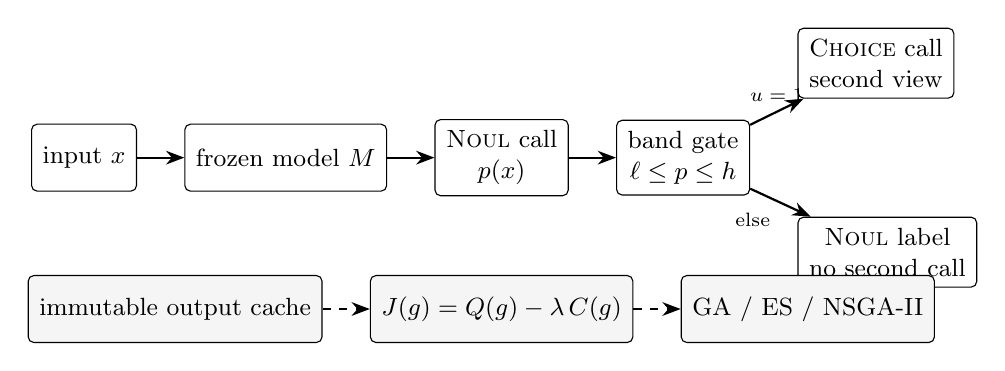
\begin{tikzpicture}[
  font=\small,
  >=Stealth,
  node distance=6mm,
  box/.style={draw, rounded corners=2pt, align=center, inner sep=4pt,
              minimum height=8.5mm, fill=white},
  arr/.style={->, thick},
  dashedarr/.style={->, thick, dashed}
]
\node[box] (x) {input $x$};
\node[box, right=of x] (m) {frozen model $M$};
\node[box, right=of m] (p) {\noul{} call\\$p(x)$};
\node[box, right=of p] (g) {band gate\\$\ell \le p \le h$};
\node[box, right=of g, yshift=12mm] (c) {\choice{} call\\second view};
\node[box, right=of g, yshift=-12mm] (n) {\noul{} label\\no second call};
\draw[arr] (x) -- (m);
\draw[arr] (m) -- (p);
\draw[arr] (p) -- (g);
\draw[arr] (g) -- node[above, font=\scriptsize]{$u=1$} (c);
\draw[arr] (g) -- node[below left, font=\scriptsize]{else} (n);
\node[box, below=10mm of p, fill=gray!8] (fit) {$J(g)=Q(g)-\lambda\,C(g)$};
\node[box, left=of fit, fill=gray!8] (cache) {immutable output cache};
\node[box, right=of fit, fill=gray!8] (search) {GA / ES / NSGA-II};
\draw[dashedarr] (cache) -- (fit);
\draw[dashedarr] (fit) -- (search);
\end{tikzpicture}
\caption{The routing setting. A frozen model answers a first \noul{} question;
a two-parameter gate decides whether the same model is asked a second
\choice{} question. Search operates entirely on cached outputs: a candidate
genome is scored by replaying the cache, and the optimiser only sees the scalar
fitness $J$. The dashed path is offline; the solid path is the deployed policy.}
\label{fig:pipeline}
\end{figure*}

For the binary tasks, CodeXGLUE and FinDVer, the first action is \noul{}: the
model answers a yes/no question and returns $p(x)=P(\text{true}\mid x)$. The
second action is \choice{}: the model selects between two named labels. In
CodeXGLUE the questions are whether a function contains a vulnerability and
whether it should be labelled \texttt{secure} or \texttt{vulnerable}; in
FinDVer they are whether a claim is supported and whether it should be labelled
\texttt{supported} or \texttt{not supported}. The cascade always pays for
\noul{} first and pays for \choice{} only when the gate opens. A policy is a
genome $g_{\mathrm{cas}}=(\ell,h,u)$ with $\ell,h\in[0,1]$ and
$u\in\{0,1\}$:
\begin{equation}
\pi_{g}(x)=
\begin{cases}
\choice(x), & u=1\!\land\!\ell\le p(x)\le h,\\
\noul(x), & \text{otherwise}.
\end{cases}
\label{eq:cascade}
\end{equation}
The gate uses the positive-class probability rather than symmetric confidence,
because a \noul{} question has a designated true label. Genome repair clips
$\ell$ and $h$ to $[0,1]$, swaps them when $\ell>h$, and maps $u$ to $\{0,1\}$.
Two fixed policies are special cases: $u=0$ is \noul-only, and
$u=1,\ell=0,h=1$ is fixed switch-only, which still pays for the first \noul{}
call and therefore costs two calls per row.

ProcessBench has a different action space. The model returns a ranked list of
candidate steps, and the policy decides whether to answer with the top-1 step or
to abstain. A genome $g_{\mathrm{abs}}=(t,v,m)$ with $t,m\in[0,1]$ and
$v\in\{0,1\}$ uses the top-1 probability $s_1(x)$ and the top-1/top-2 margin
$\Delta(x)$:
\begin{equation}
\mathrm{abstain}(x)=
\begin{cases}
\text{true}, & s_1(x)<t,\\
\text{true}, & v=1\,\land\,\Delta(x)<m,\\
\text{false}, & \text{otherwise}.
\end{cases}
\label{eq:abstain}
\end{equation}
When the required confidence fields are missing, the evaluator fails closed:
the row is forced to answer and is counted as incorrect rather than silently
dropped. We report coverage (the fraction of rows answered) and selective
accuracy (accuracy on answered rows).

Fitness combines task quality with the cost of the second call:
\begin{equation}
J(g)=Q(g)-\lambda\,C(g),
\label{eq:fitness}
\end{equation}
where $Q$ is macro-F1 on the binary tasks and step accuracy on ProcessBench,
$C(g)$ is the mean number of model calls per row minus one, and $\lambda=0.05$
is fixed before search. Macro-F1 is primary because both binary datasets are
class-imbalanced; accuracy is reported alongside it. The first \noul{} call is
charged to every policy, including \noul-only, so the cost term isolates the
incremental call rather than the total inference bill. Model outputs are
generated once and replayed from an immutable JSON cache, which makes candidate
evaluation deterministic and cheap.

The GA uses tournament selection, uniform crossover, Gaussian mutation and bit
flips on $u$. The ES is a $(\mu+\lambda)$ strategy that mutates the two
endpoints and fixes $u=1$. NSGA-II maintains a non-dominated front, optimising
accuracy and negative call cost on the binary tasks and selective accuracy and
coverage on ProcessBench; because its quality objective is accuracy rather than
macro-F1, we keep its intervals separate. The main budget is 24 unique genome
evaluations with seeds 17, 23 and 41; a five-seed extension adds 59 and 73. A
probe raises the CodeXGLUE/Vela budget to 48. Random search uses the same budget
and cache.

One property of the policy class shapes the calibration experiment. The gate
depends on $p(x)$ only through the interval $\ell\le p\le h$. Any strictly
monotone transformation of $p$---temperature scaling, for example---maps the
interval to another interval and induces the same set of switched rows up to a
reparameterisation of the endpoints. A monotone recalibration therefore cannot
change the best achievable band policy on a fixed pool. It can move rows between
bands, but it cannot create a distinction between repairable and harmful rows
that the raw ordering did not already contain. Calibration and routing are
therefore evaluated separately.

\section{Experimental Design}

The experiments use three tasks whose labels and group structure are fixed
before any policy is searched. CodeXGLUE defect detection provides 21{,}854
training, 2{,}732 dev and 2{,}732 test functions; the controller pools are drawn
only from the official training split, and functions are grouped by an exact
hash of their text so that identical functions cannot cross the internal
\texttt{search\_train}, \texttt{selection\_dev} and \texttt{confirm} pools
\citep{lu2021codexglue,zhou2019devign}. Each internal pool contains 60
functions. This controls duplicate-function leakage. FinDVer provides financial claims with \texttt{supported}/\texttt{not
supported} labels; its pools are grouped by report, and contain 60, 59 and 44
claims \citep{zhao2024findver}. The official FinDVer test labels are not used
for controller search. ProcessBench contains 3{,}400 annotated records over
2{,}842 mathematical problems; its pools are grouped by problem and contain 60
records each \citep{zheng2025processbench,cobbe2021gsm8k,lightman2024verify,uesato2022process}.
FinDVer internal pools are carved from official testmini and grouped by report
(41/16/16 groups; 60/59/44 claims); labels are used inside these pools for
fitting, thresholding and frozen evaluation. The official test split is
separate and read only by the locked-test evaluator. State is a \texttt{Claim:}
line, a blank line, then an \texttt{Evidence:} block. CodeXGLUE state is raw
function text
(positive rates 0.50/0.40/0.45). ProcessBench asks ``Which step contains the
earliest error?''; its state is the problem plus \texttt{[k] step} lines and an
\texttt{ALL STEPS CORRECT} sentinel.

All inference runs on one Windows machine with CPU-only PyTorch in FP32, two
threads and one model resident at a time. Laya is pinned to source revision
\texttt{b9fe351} and checkpoint revision \texttt{7b928d8}; Vela is pinned to
revision \texttt{d6f03aa}. Peak resident memory stays below 2.2~GB. The native
single-action baselines on \texttt{search\_dev} are as follows: CodeXGLUE
accuracy is 0.450/0.650 for Laya
(\noul/\choice) and 0.633/0.667 for Vela; FinDVer is 0.712/0.644 for Laya and
0.458/0.458 for Vela; ProcessBench \choice{} accuracy is 0.10 for both models.
The near-identical per-call latency of the two representations (about
2.2--2.8~s) is why call count, rather than a model-specific latency model, is
the cost term in Equation~\ref{eq:fitness}. The native numbers already contain a warning: the better representation depends
on the task and the model, and on FinDVer the two Vela actions are
indistinguishable at the aggregate level.

The first experiment measures action complementarity without training a router. For each
task--model cell we take the better fixed action on \texttt{search\_train} and
freeze that direction; we then count rows where the alternative action repairs a
base error, rows where it breaks a correct base answer, and their difference.
The oracle headroom is the accuracy of a per-row oracle minus the accuracy of
the better fixed action. Because the direction is fixed on train, the held-out
net-repair numbers are not selected on the evaluation pool. We report net repair
in percentage points with a group-level percentile bootstrap (5{,}000
resamples), and pair it with the macro-F1 difference between fixed \choice{} and
fixed \noul{} on the same rows. ProcessBench has only one evaluated
representation, so its headroom is zero by construction and it is excluded from
the binary complementarity table.

The second experiment asks whether the signed incremental value of the second
action is predictable before that action is executed. The target is
$\Delta_i=\mathbf{1}[\choice_i\text{ correct}]-
\mathbf{1}[\noul_i\text{ correct}]\in\{-1,0,+1\}$. The features are deployable at the
moment of decision: $p$, $|p-0.5|$ and the binary entropy $-p\log p -
(1-p)\log(1-p)$; no \choice{} output, gold label or downstream feature is used.
We compare logistic regression, a shallow decision tree, a single confidence
threshold and a never-switch majority baseline. Training uses group-aware
three-fold out-of-fold predictions; the predictor and threshold are then chosen
together on \texttt{selection\_dev} by cost-adjusted net utility, frozen, and
evaluated once on \texttt{confirm}. Net utility is (repairs $-$ regressions)
divided by the number of rows; the cost-adjusted variant subtracts
$\lambda=0.05$ per switch. A champion that switches every row is retained, because it reveals
whether the predictor adds anything beyond fixed switching.

The search comparison runs optimisers under a matched evaluation budget. GA, ES and NSGA-II
are run on the cached pools with 24 unique genome evaluations and seeds 17, 23
and 41; the five-seed extension adds 59 and 73. Random search receives the same
budget. The primary deployment comparison is pre-specified: the GA genome
selected on \texttt{search\_train} is frozen and compared with fixed
switch-only on \texttt{confirm} using paired group-bootstrap macro-F1 intervals.
All other cell-level comparisons are exploratory and are reported with effect
estimates and intervals rather than as significance claims. We then examine the
search trajectory itself: best-so-far fitness per generation, the number of
unique genomes actually evaluated, the fraction of single-gene mutations that
leave fitness unchanged, the rank correlation between train and dev fitness
across the archive, and the effect of raising the budget cap from 24 to 48 on
CodeXGLUE with Vela.

Two boundary checks test whether the conclusions generalise. The transfer experiment freezes each source-task
genome and applies it to every target task and pool without re-searching;
diagonal cells are same-task deployment checks, off-diagonal cells are true
transfer. The fault map partitions rows by task, model and a confidence band
derived from \noul{} probability or candidate margin, and reports the error
severity of each cell on discover, dev and confirm. A cell is eligible when it
contains at least eight rows on the discover pool, and it is confirmed when the
dev or confirm severity is within 0.15 of the discover severity.

Two statistical details matter for reading the tables. All binary comparisons
use paired group bootstrap with 5{,}000 resamples and a fixed random state
\citep{efron1993bootstrap}; the resampling unit is the group (function hash or
report), not the row, so dependence within a report is preserved. We report
McNemar exact tests for repair/harmful counts \citep{mcnemar1947} and Wilson
intervals for within-cell severity \citep{wilson1927}, but we do not call a
result significant on the basis of a single seed or a single pool. The locked
test was run once under a protocol frozen before any test call. The confirm
pools are held out from search and threshold selection but have been inspected
during analysis.

\section{Results and Discussion}
\label{sec:results}

The first question is whether the action set offers anything to route. Table
\ref{tab:complementarity} and Figure~\ref{fig:headroom}
(Appendix~\ref{app:extra}) answer it at the level of individual rows. Gross
complementarity is not scarce. On CodeXGLUE with Laya, \choice{} repairs 14 of
the 60 \noul{} errors, and the per-row oracle reaches 0.783 accuracy against
0.550 for the better fixed action, a headroom of 0.233. The same cell shows why
headroom is a poor promise: \choice{} breaks 15 correct \noul{} answers, so the
net count on the training pool is $-1$ and the net-repair interval spans zero.
The other three binary cells have smaller gross opportunities (headroom
0.067--0.100) and net counts between $-6$ and $+1$. Across the four cells, the
training pool never produces a net repair distinguishable from zero.

Held-out pools do not turn the gross opportunity into a stable net gain. The
CodeXGLUE/Laya cell gains 20.0 points on \texttt{selection\_dev}
($[+1.7,+38.3]$), but the same frozen direction gains only 1.7 points on confirm
($[-18.3,+20.0]$). That gap is a selection-pool effect, not a routing effect:
dev is the pool on which the direction was chosen. FinDVer with Laya is the
exception that tests the narrative. Its confirm net repair is $+13.6$ points
$[+2.0,+24.6]$, and the fixed-action accuracy difference is $+0.136$
$[+0.020,+0.246]$. The corresponding macro-F1 difference, however, is $+0.111$
with an interval that crosses zero, and the better fixed action reverses from
\noul{} on dev to \choice{} on confirm. The cell therefore contains a real
accuracy-level repair signal on confirm, but not a macro-F1 gain, and not a
direction that a train-selected policy could have known to exploit. CodeXGLUE
with Vela moves the other way: the frozen direction is \choice{}-to-\noul{},
the train net is $-6$, and confirm is exactly zero. FinDVer with Vela is negative
on confirm ($-2.3$ points). Complementarity exists in the action set, but it is
sparse, metric-dependent and pool-dependent.

\input{tables/tab_complementarity}

The location of the repairs matters as much as their count. Figure
\ref{fig:repair} (Appendix~\ref{app:extra}) plots the repair rate against the
\noul{} probability bin. Repairs concentrate in the middle and high bands,
around $p\in[0.4,0.8]$, and are close to zero in the lowest band. This is the
opposite of what a confidence cascade assumes: a threshold rule switches when
the model is uncertain, which is precisely where \choice{} is least likely to
fix anything, because the rows it can repair are rows where \noul{} was
confident and wrong. It also explains why calibration cannot rescue the router:
recalibration moves probability mass monotonically, but it does not move
repairable rows from the middle of the distribution to the low-confidence tail.

The second question is whether the incremental value of \choice{} is
predictable from the first call. Table~\ref{tab:predictability} reports
out-of-fold ranking quality and the net utility of the frozen dev-selected
policy. Ranking quality varies widely. Logistic regression reaches 0.674 on
CodeXGLUE with Laya and 0.919 on FinDVer with Vela; the tree reaches 0.739 on
CodeXGLUE with Laya. On FinDVer with Laya both predictors are near chance (0.455
and 0.466), unsurprising given that the cell has only five training repairs. The
policy results are weaker than the ranking results. The best dev policy for
CodeXGLUE with Laya is logistic regression with a threshold that switches every
row: dev net $+20.0$ points, confirm net $+1.7$ points and a cost-adjusted
$-3.3$. The FinDVer/Vela cell, despite the highest OOF AUROC, chooses a policy
with dev net $+3.4$ and confirm net $-2.3$ (zero repairs, one regression).
FinDVer with Laya selects a tree that switches one row and gains 2.3 points on
confirm, a point estimate built on a single decision. CodeXGLUE with Vela is
positive on dev ($+3.3$) and negative on confirm ($-1.7$). In no cell does a
high ranking score translate into a confirm net utility that is both positive
and estimated with enough support to matter.

\input{tables/tab_predictability}

Calibration is the most natural explanation for a failed probability-based
router, so it serves as a control. Table~\ref{tab:calibration} and
Figure~\ref{fig:calibration} in Appendix~\ref{app:extra} show that raw
probabilities are poorly calibrated on confirm: ECE ranges from 0.090 to 0.290
and Brier scores from 0.218 to 0.287. Temperature scaling, fitted on
\texttt{search\_train}, reduces ECE in three of four cells (to 0.045--0.169) and
Brier in all four. Routing is unaffected: raw probabilities give confirm net
repairs of $-5.0$, $0.0$, $+2.3$ and $-2.3$ points, temperature-scaled ones give
$-1.7$, $+1.7$, $0.0$ and $0.0$, as the invariance argument in
Section~\ref{sec:method} predicts. The repair AUROC makes the point directly:
0.791, 0.444, 0.336 and 0.095 for the four cells; in the last two the
probability ranks repairable rows \emph{below} chance. A calibrated probability
of the current answer is not a calibrated probability of the alternative
action's value.

The third question is whether search converts the available signal into a
deployable policy. Table~\ref{tab:search} summarises the comparison. GA versus
random search is the cleanest test of optimiser value: with five seeds, four
task--model cells and three pools, there are 60 paired macro-F1 comparisons, and
none has an interval that excludes zero. GA versus fixed switch-only has five
significant positive cells, all on the FinDVer/Vela training pool and all with
an effect near $+0.12$; on dev and confirm, none of the 40 comparisons is
significant. The pre-registered deployment comparison---train-selected GA
against fixed switch-only on confirm---is null in every seed-level cell. ES
versus random search is null in all 30 comparisons; ES versus fixed switching
has three significant training cells and one significant confirm cell
(CodeXGLUE/Laya, seed 17, $+0.176$), the only confirm-level positive result, and
it is not replicated across seeds. NSGA-II deployment is significantly worse
than the fixed baseline in five dev cells and one confirm cell, with no positive
cell. The search problem has no stable held-out signal for any optimiser to
find.

\input{tables/tab_search}

The trajectory diagnostics explain why more search does not help. In 15 of 21
logged GA/ES runs, best-so-far fitness does not improve after generation zero.
The neutral-mutation rate is 0.68--0.73, so most mutations produce a candidate
with exactly the same training score. The train--dev rank correlation is $-0.56$
and $-0.51$ for the two CodeXGLUE cells, meaning that candidates which look
better on train tend to look worse on dev, and $+0.44$ and $+0.99$ for the
FinDVer cells. Raising the budget from 24 to 48 on CodeXGLUE with Vela does not
close the gap: the GA evaluates only 22, 17 and 23 unique genomes under a cap of
48, while random search uses all 48. The search is not merely under-tuned; it is
under-informed.

The boundary checks ask whether these conclusions are artefacts of one pool or
task. Appendix~\ref{app:boundary} reports the transfer table and fault map.
Transfer is uniformly unhelpful: of 32 source--target by split units, six have a
significant paired difference against the target's fixed switch policy, and all
six are negative (two diagonal, four off-diagonal). The fault map is more
nuanced: of 15 eligible cells, 13 are confirmed on dev and 10 on confirm. The
highest confirm severities are on ProcessBench (Vela/mid 0.833, Laya/mid 0.875,
Vela/low 0.936, Laya/high 0.895). The mid-confidence cells are not simply the
low-confidence tail: a model can be moderately confident and still fail, and the
second representation fails on the same rows, so no gate on the first action's
probability can create a repair.

Taken together, the three questions describe a routing problem that fails before
the optimiser is asked to solve it: RQ1 finds gross but no stable net
complementarity, RQ2 finds ranking signal without reliable policy value, and RQ3
finds no held-out advantage because the landscape is flat and the training
ranking does not predict the dev ranking where it matters. Calibration improves
a different quantity: a model can report better probabilities for the question
it answered and still have nothing to say about whether a different question
would be answered better.

The practical implication is a change in the order of work. Before building a
router, measure whether the action set has net complementarity on held-out
groups and whether the candidate features rank repairable rows above chance. If
either check fails, a stronger optimiser will not help; if both pass, the
optimiser comparison can be run under a matched budget with a pre-registered
confirm comparison.

\section{Conclusion}

A probability returned with every typed judgment should decide when a second
judgment is worth buying. Our experiments on frozen Laya and Vela across three
tasks do not support that promise: evolutionary search produces no held-out
advantage over fixed policies or budget-matched random search.

Gross complementarity is real---a per-row oracle gains up to 23.3 accuracy
points---but harmful switches offset repairs, and the net balance is small,
metric-dependent and unstable across pools. Calibration and action-value
prediction dissociate: temperature scaling
improves ECE and Brier but not row order, and in both FinDVer cells the
probability ranks repairable rows below chance. The search landscape is flat:
most mutations are neutral, most runs plateau at generation zero, and the
training ranking does not predict the dev ranking.

Limits are part of the result: pools are small, the \noul{} template was not
audited, only two open models were run, and the locked test remains unrun. Next:
a supervision target judged by held-out net utility.

\bibliography{references}

\end{document}
"
% to obtain the camera-ready layout used by aclpubcheck.
\newif\ifaclreview
\aclreviewtrue
\ifdefined\CAMERAREADY\aclreviewfalse\fi
\ifaclreview\usepackage[review]{acl}\else\usepackage[final]{acl}\fi

\usepackage{times}
\usepackage{latexsym}
\usepackage[T1]{fontenc}
\usepackage[utf8]{inputenc}
\usepackage{microtype}
\usepackage{inconsolata}
\usepackage{graphicx}
\usepackage{capt-of}
\usepackage{booktabs}
\usepackage{amsmath}
\usepackage{amssymb}
\usepackage{xcolor}
\usepackage{tikz}
\usetikzlibrary{arrows.meta,positioning}
\usepackage{url}

\setlength{\tabcolsep}{4pt}
\setlength{\textfloatsep}{8pt plus 2pt minus 2pt}
\setlength{\floatsep}{6pt plus 2pt minus 2pt}
\setlength{\intextsep}{6pt plus 2pt minus 2pt}

\newcommand{\noul}{\textsc{Noul}}
\newcommand{\choice}{\textsc{Choice}}
\newcommand{\score}{\textsc{Score}}
\newcommand{\spanact}{\textsc{Span}}
\newcommand{\setact}{\textsc{Set}}
\newcommand{\eg}{e.g.,}
\newcommand{\ie}{i.e.,}

\title{When Evolutionary Routing Fails:\\ Action Complementarity and Utility Prediction in Structured Decision Models}

\author{Anonymous ACL submission}

\begin{document}
\maketitle

\begin{abstract}
Structured decision models such as Jev turn a language-model call into a typed
probabilistic judgment: a binary \noul{} decision, a candidate \choice{}, or a
\score{}. This interface makes inference-time routing attractive: ask a cheap
\noul{} question first and buy a second, differently framed \choice{} view only
when the first answer looks uncertain. We test that intuition with frozen open
models. Using Laya 0.4.16 and Vela 2.0 0.3B on CodeXGLUE defect detection,
FinDVer claim verification and ProcessBench reasoning-error localisation, we
compare a genetic algorithm, an evolution strategy and NSGA-II with fixed
policies and budget-matched random search, and measure per-example action
complementarity and the predictability of the second action's signed
incremental utility. Gross repair opportunities exist: a per-row oracle gains
up to 23.3 accuracy points over the better fixed action. Net repair is sparse
and pool-dependent: only one of four confirm cells has a positive accuracy
interval, and its macro-F1 interval still spans zero. Out-of-fold rank
correlation for a signed-utility predictor is weak ($|\text{Spearman}|\le
0.19$; every group-bootstrap interval includes zero), and confirm cost-adjusted
utility is non-positive in all four cells. No genetic-algorithm genome beats
the better fixed action, including on a one-shot locked test; the only
locked-test gain is over the worse fixed switch, where it learns to stay on
\noul{}. Calibration improves probabilities but does not create routing signal,
because monotone recalibration leaves the band policy class unchanged.
\end{abstract}

\section{Introduction}

A claims analyst asks a model whether a sentence is supported by a financial
report; a security engineer asks whether a C function contains a vulnerability;
a mathematician asks where the first invalid step occurs. Each case needs a
decision that software can branch on without a second interpretation step.
System One models answer that demand directly. Given a state and a typed
question, Jev returns a binary \noul{}, a candidate \choice{}, or an ordered
\score{} with probabilities \citep{typesafe2026,deusser2026jev}; Laya and Vela
expose similar interfaces in open weights \citep{laya2026,vllm2026vela}.

The interface suggests a simple policy. Ask the cheap binary question first,
read the returned probability, and spend a second call on a differently framed
\choice{} question only when the first answer looks uncertain. The policy is
easy to deploy and matches how practitioners use confidence thresholds. It also
assumes that the probability of the current answer predicts the value of a
different answer. That assumption does not follow from the training objective.
RLCD, the recipe behind Jev and the one Laya documents, rewards honest
probabilities for the question the model answered
\citep{typesafe2026,laya2026,gneiting2007scoring}. A calibrated head can
therefore coexist with a router that has no useful signal. Cascades face the
same limit: confidence-based deferral is optimal only when downstream errors
are tied to upstream confidence, and specialised errors, label noise or
distribution shift can break that link \citep{jitkrittum2023cascade}.

We measure the distinction. Two structured decision
models, Laya 0.4.16 and Vela 2.0 0.3B, are frozen, and routing is studied on
CodeXGLUE defect detection \citep{lu2021codexglue}, FinDVer claim verification
\citep{zhao2024findver} and ProcessBench reasoning-error localisation
\citep{zheng2025processbench}. On the binary tasks the policy pays for \noul{}
and may pay again for \choice{}; on ProcessBench it decides whether to answer or
abstain. We first measure action complementarity, then ask whether the signed
incremental value of \choice{} is predictable from the first call, and finally
compare a genetic algorithm, an evolution strategy and NSGA-II with fixed
policies and budget-matched random search. A one-shot locked test on official
test rows checks the frozen policies.

Gross complementarity is real: on CodeXGLUE, Laya gains 23.3 accuracy points
from a per-row oracle over the better fixed action, and \choice{} repairs 14
\noul{} errors. The same action breaks 15 correct answers, so the net count on
the training pool is $-1$, and held-out pools do not stabilise the sign. A
predictor trained on signed incremental utility has weak out-of-fold rank
correlation, and its confirm cost-adjusted utility is non-positive in every
cell. The genetic algorithm never significantly beats random search; on a
one-shot locked test no genome beats the better fixed action, and the only gain
is over the worse fixed switch, where it learns to stay on \noul{}.
Temperature scaling lowers calibration error but leaves the band policy class
unchanged, so it cannot create the missing signal.

The paper contributes a diagnostic decomposition of routing value into action
complementarity, signed incremental-utility prediction and search efficacy,
measured on frozen structured decision models rather than inferred from
end-task accuracy. It reports a pre-specified negative result across five seeds,
three pools and four task--model cells, and it shows that calibration and
action-value prediction dissociate. The practical lesson is to measure net
complementarity and the predictability of the alternative action before
building a router; a stronger optimiser cannot recover a signal the action set
does not contain.

\section{Background and Related Work}

Structured decision models replace free-form generation with a typed question
and a typed answer. Jev, the commercial System One model from TypeSafe, accepts
a state and a set of questions and returns \noul{} (a binary judgment),
\choice{} (a selection among named candidates) or \score{} (an ordered rating)
with associated probabilities \citep{typesafe2026}. \citet{deusser2026jev}
benchmark Jev on 37 datasets, and \citet{guo2026justask} apply it to alignment
failure detection; both treat the model as a general decision interface rather
than a text generator. TypeSafe describes the training objective as
Reinforcement Learning for Calibrated Decisions (RLCD), which optimises the
reported distribution with strictly proper scoring rules so that probabilities
carry information beyond the argmax; the full recipe is not public.
\citet{gao2026openjev} provide an independent open implementation. The name
RLCD also appears in \citet{yang2023rlcd} for Reinforcement Learning from
Contrast Distillation; the two are unrelated, and we use RLCD only in the
calibrated-decision sense.

The two models we run differ in backbone and supervision while sharing the
interface. Laya 0.4.16 is a ModernBERT-large encoder with decision-specific
heads, about 421M parameters, and supports \noul{}, \choice{} and \score{} in a
non-autoregressive pass; it is the open model closest to the RLCD description
\citep{laya2026,layastudio2026}. Vela 2.0 0.3B is a 22-layer ModernBERT encoder
with an 8{,}192-token window; it exposes the same three actions plus \spanact{}
and \setact{}, and was initialised from the Decision-1.0-Kai \choice{} path with
task-specific losses and routing data \citep{vllm2026vela,warner2024modernbert}.
Vela's card does not call the recipe RLCD, so we treat Laya as an open RLCD
model and Vela as an interface-matched comparison with a different training
route (Appendix~\ref{app:models}).

Calibration is the natural first lens on these probabilities. Neural networks
are often overconfident, and temperature scaling or other post-hoc maps can
reduce expected calibration error without changing the argmax
\citep{guo2017calibration}. Language models can also partially recognise their
own errors, which makes confidence a plausible routing feature
\citep{kadavath2022know}, and proper scoring rules formalise why a reported
probability should be rewarded for honesty rather than sharpness alone
\citep{gneiting2007scoring}. All of this work concerns the probability of the
answer the model has already produced, not whether that probability orders the
counterfactual value of a different question type. We measure ECE and Brier for
current-answer correctness, then measure the same probability's ability to rank
rows that the alternative action would repair.

Cascades and routers allocate computation across models or actions. The
classical cascade rejects easy examples early and sends hard ones to a stronger
classifier \citep{viola2001rapid}; modern systems learn when to call a larger
language model \citep{chen2024frugalgpt,aggarwal2024automix,ong2024routellm},
how many candidates to sample \citep{ding2025bestroute}, or how to combine
routing and cascading in one objective \citep{dekoninck2025unified}. The
theoretical caution comes from \citet{jitkrittum2023cascade}: confidence-based
deferral is optimal only when downstream errors are sufficiently tied to
upstream confidence, and it can fail under specialised downstream errors, label
noise or distribution shift. \citet{damani2025hard} argue that computation should
follow expected benefit rather than surface difficulty. Our experiments
instantiate this warning in a structured decision model: the second action is a
different question to the same frozen network, not a larger model, and its value
depends on an error structure that the first probability does not encode. For
ProcessBench, selective prediction supplies the abstention framing:
\citet{chow1970optimum} derives the optimal reject rule under known
distributions, and \citet{geifman2017selective}, \citet{kamath2020selective} and
\citet{xin2021art} study selective classification, question answering and the
separation of coverage from conditional accuracy.

Evolutionary methods are a reasonable choice when the policy is a small
non-differentiable object and the objective is a cached replay. Genetic
algorithms, evolution strategies and NSGA-II cover single-objective and Pareto
formulations \citep{deb2002nsga2,hansen2001cmaes,stanley2002neat}, and
regularised evolution has been used for architecture search
\citep{real2019regularized,elsken2019nas}. In NLP, EvoPrompt and Promptbreeder
evolve prompts or mutation instructions with language models in the loop
\citep{guo2024evoprompt,fernando2024promptbreeder}. Those systems search over
text that changes what the model sees; we hold the model and the question
template fixed and search over a two-parameter gate that decides whether a
second typed question is asked. Prompt search can improve a single call, whereas
our search can only exploit complementarity that already exists between two
fixed actions. A flat landscape is therefore a finding about the action set, not
merely about optimiser strength.

Our protocol follows the variance-aware reporting practices of
\citet{henderson2018matters}, \citet{bouthillier2021variance} and
\citet{dodge2019show}: we fix the action set, templates and budget before
looking at confirm, report every seed-level interval rather than only the best
cell, and label the locked test as not run rather than substituting a confirm
number for it.

\section{Method and Decision Rules}
\label{sec:method}

We study a frozen model $M$ and a fixed action set $\mathcal{A}$. An input $x$
is rendered by a task adapter into a state string and a typed question; the
model returns a schema-validated decision with a probability. The policy reads
only the first call and decides whether to issue a second call. Model weights,
question templates and candidate label sets are never modified during search.
This isolates inference-time control from fine-tuning the backbone on the
routing objective.

\begin{figure*}[t]
\centering
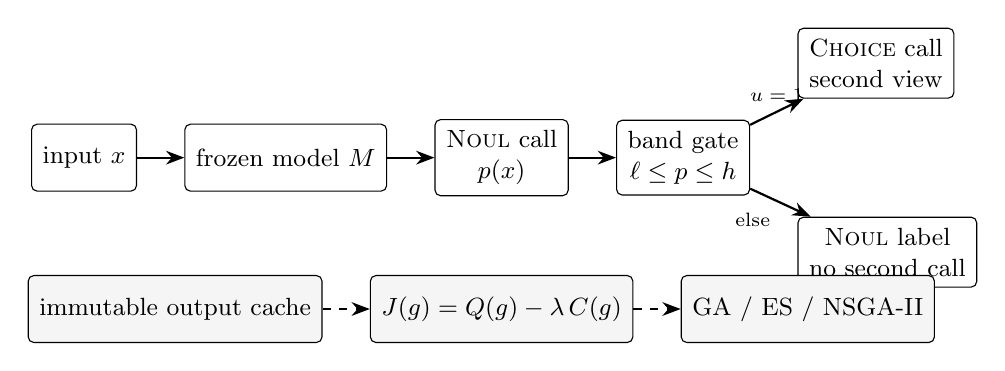
\begin{tikzpicture}[
  font=\small,
  >=Stealth,
  node distance=6mm,
  box/.style={draw, rounded corners=2pt, align=center, inner sep=4pt,
              minimum height=8.5mm, fill=white},
  arr/.style={->, thick},
  dashedarr/.style={->, thick, dashed}
]
\node[box] (x) {input $x$};
\node[box, right=of x] (m) {frozen model $M$};
\node[box, right=of m] (p) {\noul{} call\\$p(x)$};
\node[box, right=of p] (g) {band gate\\$\ell \le p \le h$};
\node[box, right=of g, yshift=12mm] (c) {\choice{} call\\second view};
\node[box, right=of g, yshift=-12mm] (n) {\noul{} label\\no second call};
\draw[arr] (x) -- (m);
\draw[arr] (m) -- (p);
\draw[arr] (p) -- (g);
\draw[arr] (g) -- node[above, font=\scriptsize]{$u=1$} (c);
\draw[arr] (g) -- node[below left, font=\scriptsize]{else} (n);
\node[box, below=10mm of p, fill=gray!8] (fit) {$J(g)=Q(g)-\lambda\,C(g)$};
\node[box, left=of fit, fill=gray!8] (cache) {immutable output cache};
\node[box, right=of fit, fill=gray!8] (search) {GA / ES / NSGA-II};
\draw[dashedarr] (cache) -- (fit);
\draw[dashedarr] (fit) -- (search);
\end{tikzpicture}
\caption{The routing setting. A frozen model answers a first \noul{} question;
a two-parameter gate decides whether the same model is asked a second
\choice{} question. Search operates entirely on cached outputs: a candidate
genome is scored by replaying the cache, and the optimiser only sees the scalar
fitness $J$. The dashed path is offline; the solid path is the deployed policy.}
\label{fig:pipeline}
\end{figure*}

For the binary tasks, CodeXGLUE and FinDVer, the first action is \noul{}: the
model answers a yes/no question and returns $p(x)=P(\text{true}\mid x)$. The
second action is \choice{}: the model selects between two named labels. In
CodeXGLUE the questions are whether a function contains a vulnerability and
whether it should be labelled \texttt{secure} or \texttt{vulnerable}; in
FinDVer they are whether a claim is supported and whether it should be labelled
\texttt{supported} or \texttt{not supported}. The cascade always pays for
\noul{} first and pays for \choice{} only when the gate opens. A policy is a
genome $g_{\mathrm{cas}}=(\ell,h,u)$ with $\ell,h\in[0,1]$ and
$u\in\{0,1\}$:
\begin{equation}
\pi_{g}(x)=
\begin{cases}
\choice(x), & u=1\!\land\!\ell\le p(x)\le h,\\
\noul(x), & \text{otherwise}.
\end{cases}
\label{eq:cascade}
\end{equation}
The gate uses the positive-class probability rather than symmetric confidence,
because a \noul{} question has a designated true label. Genome repair clips
$\ell$ and $h$ to $[0,1]$, swaps them when $\ell>h$, and maps $u$ to $\{0,1\}$.
Two fixed policies are special cases: $u=0$ is \noul-only, and
$u=1,\ell=0,h=1$ is fixed switch-only, which still pays for the first \noul{}
call and therefore costs two calls per row.

ProcessBench has a different action space. The model returns a ranked list of
candidate steps, and the policy decides whether to answer with the top-1 step or
to abstain. A genome $g_{\mathrm{abs}}=(t,v,m)$ with $t,m\in[0,1]$ and
$v\in\{0,1\}$ uses the top-1 probability $s_1(x)$ and the top-1/top-2 margin
$\Delta(x)$:
\begin{equation}
\mathrm{abstain}(x)=
\begin{cases}
\text{true}, & s_1(x)<t,\\
\text{true}, & v=1\,\land\,\Delta(x)<m,\\
\text{false}, & \text{otherwise}.
\end{cases}
\label{eq:abstain}
\end{equation}
When the required confidence fields are missing, the evaluator fails closed:
the row is forced to answer and is counted as incorrect rather than silently
dropped. We report coverage (the fraction of rows answered) and selective
accuracy (accuracy on answered rows).

Fitness combines task quality with the cost of the second call:
\begin{equation}
J(g)=Q(g)-\lambda\,C(g),
\label{eq:fitness}
\end{equation}
where $Q$ is macro-F1 on the binary tasks and step accuracy on ProcessBench,
$C(g)$ is the mean number of model calls per row minus one, and $\lambda=0.05$
is fixed before search. Macro-F1 is primary because both binary datasets are
class-imbalanced; accuracy is reported alongside it. The first \noul{} call is
charged to every policy, including \noul-only, so the cost term isolates the
incremental call rather than the total inference bill. Model outputs are
generated once and replayed from an immutable JSON cache, which makes candidate
evaluation deterministic and cheap.

The GA uses tournament selection, uniform crossover, Gaussian mutation and bit
flips on $u$. The ES is a $(\mu+\lambda)$ strategy that mutates the two
endpoints and fixes $u=1$. NSGA-II maintains a non-dominated front, optimising
accuracy and negative call cost on the binary tasks and selective accuracy and
coverage on ProcessBench; because its quality objective is accuracy rather than
macro-F1, we keep its intervals separate. The main budget is 24 unique genome
evaluations with seeds 17, 23 and 41; a five-seed extension adds 59 and 73. A
probe raises the CodeXGLUE/Vela budget to 48. Random search uses the same budget
and cache.

One property of the policy class shapes the calibration experiment. The gate
depends on $p(x)$ only through the interval $\ell\le p\le h$. Any strictly
monotone transformation of $p$---temperature scaling, for example---maps the
interval to another interval and induces the same set of switched rows up to a
reparameterisation of the endpoints. A monotone recalibration therefore cannot
change the best achievable band policy on a fixed pool. It can move rows between
bands, but it cannot create a distinction between repairable and harmful rows
that the raw ordering did not already contain. Calibration and routing are
therefore evaluated separately.

\section{Experimental Design}

The experiments use three tasks whose labels and group structure are fixed
before any policy is searched. CodeXGLUE defect detection provides 21{,}854
training, 2{,}732 dev and 2{,}732 test functions; the controller pools are drawn
only from the official training split, and functions are grouped by an exact
hash of their text so that identical functions cannot cross the internal
\texttt{search\_train}, \texttt{selection\_dev} and \texttt{confirm} pools
\citep{lu2021codexglue,zhou2019devign}. Each internal pool contains 60
functions. This controls duplicate-function leakage. FinDVer provides financial claims with \texttt{supported}/\texttt{not
supported} labels; its pools are grouped by report, and contain 60, 59 and 44
claims \citep{zhao2024findver}. The official FinDVer test labels are not used
for controller search. ProcessBench contains 3{,}400 annotated records over
2{,}842 mathematical problems; its pools are grouped by problem and contain 60
records each \citep{zheng2025processbench,cobbe2021gsm8k,lightman2024verify,uesato2022process}.
FinDVer internal pools are carved from official testmini and grouped by report
(41/16/16 groups; 60/59/44 claims); labels are used inside these pools for
fitting, thresholding and frozen evaluation. The official test split is
separate and read only by the locked-test evaluator. State is a \texttt{Claim:}
line, a blank line, then an \texttt{Evidence:} block. CodeXGLUE state is raw
function text
(positive rates 0.50/0.40/0.45). ProcessBench asks ``Which step contains the
earliest error?''; its state is the problem plus \texttt{[k] step} lines and an
\texttt{ALL STEPS CORRECT} sentinel.

All inference runs on one Windows machine with CPU-only PyTorch in FP32, two
threads and one model resident at a time. Laya is pinned to source revision
\texttt{b9fe351} and checkpoint revision \texttt{7b928d8}; Vela is pinned to
revision \texttt{d6f03aa}. Peak resident memory stays below 2.2~GB. The native
single-action baselines on \texttt{search\_dev} are as follows: CodeXGLUE
accuracy is 0.450/0.650 for Laya
(\noul/\choice) and 0.633/0.667 for Vela; FinDVer is 0.712/0.644 for Laya and
0.458/0.458 for Vela; ProcessBench \choice{} accuracy is 0.10 for both models.
The near-identical per-call latency of the two representations (about
2.2--2.8~s) is why call count, rather than a model-specific latency model, is
the cost term in Equation~\ref{eq:fitness}. The native numbers already contain a warning: the better representation depends
on the task and the model, and on FinDVer the two Vela actions are
indistinguishable at the aggregate level.

The first experiment measures action complementarity without training a router. For each
task--model cell we take the better fixed action on \texttt{search\_train} and
freeze that direction; we then count rows where the alternative action repairs a
base error, rows where it breaks a correct base answer, and their difference.
The oracle headroom is the accuracy of a per-row oracle minus the accuracy of
the better fixed action. Because the direction is fixed on train, the held-out
net-repair numbers are not selected on the evaluation pool. We report net repair
in percentage points with a group-level percentile bootstrap (5{,}000
resamples), and pair it with the macro-F1 difference between fixed \choice{} and
fixed \noul{} on the same rows. ProcessBench has only one evaluated
representation, so its headroom is zero by construction and it is excluded from
the binary complementarity table.

The second experiment asks whether the signed incremental value of the second
action is predictable before that action is executed. The target is
$\Delta_i=\mathbf{1}[\choice_i\text{ correct}]-
\mathbf{1}[\noul_i\text{ correct}]\in\{-1,0,+1\}$. The features are deployable at the
moment of decision: $p$, $|p-0.5|$ and the binary entropy $-p\log p -
(1-p)\log(1-p)$; no \choice{} output, gold label or downstream feature is used.
We compare logistic regression, a shallow decision tree, a single confidence
threshold and a never-switch majority baseline. Training uses group-aware
three-fold out-of-fold predictions; the predictor and threshold are then chosen
together on \texttt{selection\_dev} by cost-adjusted net utility, frozen, and
evaluated once on \texttt{confirm}. Net utility is (repairs $-$ regressions)
divided by the number of rows; the cost-adjusted variant subtracts
$\lambda=0.05$ per switch. A champion that switches every row is retained, because it reveals
whether the predictor adds anything beyond fixed switching.

The search comparison runs optimisers under a matched evaluation budget. GA, ES and NSGA-II
are run on the cached pools with 24 unique genome evaluations and seeds 17, 23
and 41; the five-seed extension adds 59 and 73. Random search receives the same
budget. The primary deployment comparison is pre-specified: the GA genome
selected on \texttt{search\_train} is frozen and compared with fixed
switch-only on \texttt{confirm} using paired group-bootstrap macro-F1 intervals.
All other cell-level comparisons are exploratory and are reported with effect
estimates and intervals rather than as significance claims. We then examine the
search trajectory itself: best-so-far fitness per generation, the number of
unique genomes actually evaluated, the fraction of single-gene mutations that
leave fitness unchanged, the rank correlation between train and dev fitness
across the archive, and the effect of raising the budget cap from 24 to 48 on
CodeXGLUE with Vela.

Two boundary checks test whether the conclusions generalise. The transfer experiment freezes each source-task
genome and applies it to every target task and pool without re-searching;
diagonal cells are same-task deployment checks, off-diagonal cells are true
transfer. The fault map partitions rows by task, model and a confidence band
derived from \noul{} probability or candidate margin, and reports the error
severity of each cell on discover, dev and confirm. A cell is eligible when it
contains at least eight rows on the discover pool, and it is confirmed when the
dev or confirm severity is within 0.15 of the discover severity.

Two statistical details matter for reading the tables. All binary comparisons
use paired group bootstrap with 5{,}000 resamples and a fixed random state
\citep{efron1993bootstrap}; the resampling unit is the group (function hash or
report), not the row, so dependence within a report is preserved. We report
McNemar exact tests for repair/harmful counts \citep{mcnemar1947} and Wilson
intervals for within-cell severity \citep{wilson1927}, but we do not call a
result significant on the basis of a single seed or a single pool. The locked
test was run once under a protocol frozen before any test call. The confirm
pools are held out from search and threshold selection but have been inspected
during analysis.

\section{Results and Discussion}
\label{sec:results}

The first question is whether the action set offers anything to route. Table
\ref{tab:complementarity} and Figure~\ref{fig:headroom}
(Appendix~\ref{app:extra}) answer it at the level of individual rows. Gross
complementarity is not scarce. On CodeXGLUE with Laya, \choice{} repairs 14 of
the 60 \noul{} errors, and the per-row oracle reaches 0.783 accuracy against
0.550 for the better fixed action, a headroom of 0.233. The same cell shows why
headroom is a poor promise: \choice{} breaks 15 correct \noul{} answers, so the
net count on the training pool is $-1$ and the net-repair interval spans zero.
The other three binary cells have smaller gross opportunities (headroom
0.067--0.100) and net counts between $-6$ and $+1$. Across the four cells, the
training pool never produces a net repair distinguishable from zero.

Held-out pools do not turn the gross opportunity into a stable net gain. The
CodeXGLUE/Laya cell gains 20.0 points on \texttt{selection\_dev}
($[+1.7,+38.3]$), but the same frozen direction gains only 1.7 points on confirm
($[-18.3,+20.0]$). That gap is a selection-pool effect, not a routing effect:
dev is the pool on which the direction was chosen. FinDVer with Laya is the
exception that tests the narrative. Its confirm net repair is $+13.6$ points
$[+2.0,+24.6]$, and the fixed-action accuracy difference is $+0.136$
$[+0.020,+0.246]$. The corresponding macro-F1 difference, however, is $+0.111$
with an interval that crosses zero, and the better fixed action reverses from
\noul{} on dev to \choice{} on confirm. The cell therefore contains a real
accuracy-level repair signal on confirm, but not a macro-F1 gain, and not a
direction that a train-selected policy could have known to exploit. CodeXGLUE
with Vela moves the other way: the frozen direction is \choice{}-to-\noul{},
the train net is $-6$, and confirm is exactly zero. FinDVer with Vela is negative
on confirm ($-2.3$ points). Complementarity exists in the action set, but it is
sparse, metric-dependent and pool-dependent.

\begin{table*}[t]
\centering
\footnotesize
\caption{Action complementarity with the train-selected direction frozen across
pools ($n=60$ per training cell; FinDVer dev/confirm: 59/44). \emph{Headroom} is the accuracy gain of a per-row
oracle over the better fixed action on \texttt{search\_train};
\emph{repair/harmful} counts rows where the alternative fixes or breaks the
base decision. Net repair is the paired difference in percentage points
(alternative minus base) with a 95\% group-bootstrap interval on dev and
confirm. Headroom is an upper bound, not a deployable gain.}
\label{tab:complementarity}
\begin{tabular}{@{}llrrrr@{}}
\toprule
Task / model & Direction & Headroom & Repair/harmful & Net dev (95\% CI) & Net confirm (95\% CI) \\
\midrule
CodeXGLUE / Laya & Noul$\to$Choice & 0.233 & 14/15 & +20.0 [+1.7, +38.3] & +1.7 [-18.3, +20.0] \\
CodeXGLUE / Vela & Choice$\to$Noul & 0.067 & 4/10 & -3.3 [-15.0, +8.3] & +0.0 [-15.0, +15.0] \\
FinDVer / Laya & Noul$\to$Choice & 0.083 & 5/6 & -6.8 [-23.3, +6.0] & +13.6 [+2.0, +24.6] \\
FinDVer / Vela & Choice$\to$Noul & 0.100 & 6/7 & +0.0 [-9.1, +11.5] & -2.3 [-10.3, +5.0] \\
\bottomrule
\end{tabular}
\end{table*}


The location of the repairs matters as much as their count. Figure
\ref{fig:repair} (Appendix~\ref{app:extra}) plots the repair rate against the
\noul{} probability bin. Repairs concentrate in the middle and high bands,
around $p\in[0.4,0.8]$, and are close to zero in the lowest band. This is the
opposite of what a confidence cascade assumes: a threshold rule switches when
the model is uncertain, which is precisely where \choice{} is least likely to
fix anything, because the rows it can repair are rows where \noul{} was
confident and wrong. It also explains why calibration cannot rescue the router:
recalibration moves probability mass monotonically, but it does not move
repairable rows from the middle of the distribution to the low-confidence tail.

The second question is whether the incremental value of \choice{} is
predictable from the first call. Table~\ref{tab:predictability} reports
out-of-fold ranking quality and the net utility of the frozen dev-selected
policy. Ranking quality varies widely. Logistic regression reaches 0.674 on
CodeXGLUE with Laya and 0.919 on FinDVer with Vela; the tree reaches 0.739 on
CodeXGLUE with Laya. On FinDVer with Laya both predictors are near chance (0.455
and 0.466), unsurprising given that the cell has only five training repairs. The
policy results are weaker than the ranking results. The best dev policy for
CodeXGLUE with Laya is logistic regression with a threshold that switches every
row: dev net $+20.0$ points, confirm net $+1.7$ points and a cost-adjusted
$-3.3$. The FinDVer/Vela cell, despite the highest OOF AUROC, chooses a policy
with dev net $+3.4$ and confirm net $-2.3$ (zero repairs, one regression).
FinDVer with Laya selects a tree that switches one row and gains 2.3 points on
confirm, a point estimate built on a single decision. CodeXGLUE with Vela is
positive on dev ($+3.3$) and negative on confirm ($-1.7$). In no cell does a
high ranking score translate into a confirm net utility that is both positive
and estimated with enough support to matter.

\begin{table*}[t]
\centering
\scriptsize
\caption{Signed incremental-utility prediction. Target
$\Delta_i=\mathbf{1}[\textsc{Choice}_i\text{ correct}]-
\mathbf{1}[\textsc{Noul}_i\text{ correct}]\in\{-1,0,+1\}$. OOF $\rho$ is the
Spearman correlation under group-aware three-fold CV on \texttt{search\_train};
the threshold is selected on \texttt{search\_dev} and frozen for
\texttt{confirm}. Net utility is mean $\Delta$ minus $\lambda=0.05$ per switch,
in points, with a 95\% group-bootstrap interval; the last column is
switches/rows.}
\label{tab:predictability}
\begin{tabular}{@{}lrrrrrr@{}}
\toprule
Task / model & OOF $\rho$ & AUROC repair & AUROC reg. & Dev net & Confirm net (95\% CI) & Switches \\
\midrule
CodeXGLUE / Laya & -0.02 & 0.360 & 0.607 & +21.7 & +0.0 [-18.8, +13.0] & 42/60 \\
CodeXGLUE / Vela & +0.19 & 0.744 & 0.335 & +3.3 & -1.7 [-19.8, +8.5] & 54/60 \\
FinDVer / Laya & +0.13 & 0.458 & 0.707 & +1.7 & +0.0 [-0.3, +0.0] & 1/44 \\
FinDVer / Vela & -0.17 & 0.396 & 0.361 & +3.4 & -2.3 [-7.7, -0.1] & 5/44 \\
\bottomrule
\end{tabular}
\end{table*}


Calibration is the most natural explanation for a failed probability-based
router, so it serves as a control. Table~\ref{tab:calibration} and
Figure~\ref{fig:calibration} in Appendix~\ref{app:extra} show that raw
probabilities are poorly calibrated on confirm: ECE ranges from 0.090 to 0.290
and Brier scores from 0.218 to 0.287. Temperature scaling, fitted on
\texttt{search\_train}, reduces ECE in three of four cells (to 0.045--0.169) and
Brier in all four. Routing is unaffected: raw probabilities give confirm net
repairs of $-5.0$, $0.0$, $+2.3$ and $-2.3$ points, temperature-scaled ones give
$-1.7$, $+1.7$, $0.0$ and $0.0$, as the invariance argument in
Section~\ref{sec:method} predicts. The repair AUROC makes the point directly:
0.791, 0.444, 0.336 and 0.095 for the four cells; in the last two the
probability ranks repairable rows \emph{below} chance. A calibrated probability
of the current answer is not a calibrated probability of the alternative
action's value.

The third question is whether search converts the available signal into a
deployable policy. Table~\ref{tab:search} summarises the comparison. GA versus
random search is the cleanest test of optimiser value: with five seeds, four
task--model cells and three pools, there are 60 paired macro-F1 comparisons, and
none has an interval that excludes zero. GA versus fixed switch-only has five
significant positive cells, all on the FinDVer/Vela training pool and all with
an effect near $+0.12$; on dev and confirm, none of the 40 comparisons is
significant. The pre-registered deployment comparison---train-selected GA
against fixed switch-only on confirm---is null in every seed-level cell. ES
versus random search is null in all 30 comparisons; ES versus fixed switching
has three significant training cells and one significant confirm cell
(CodeXGLUE/Laya, seed 17, $+0.176$), the only confirm-level positive result, and
it is not replicated across seeds. NSGA-II deployment is significantly worse
than the fixed baseline in five dev cells and one confirm cell, with no positive
cell. The search problem has no stable held-out signal for any optimiser to
find.

\begin{table}[!b]
\centering
\small
\caption{Search comparisons under the pre-specified protocol. Counts are
paired group-bootstrap 95\% intervals that exclude zero; ``positive'' means the
evolved policy beats the stated baseline. GA and ES rows use macro-F1 on all
three pools with five seeds; the NSGA-II row uses accuracy on 12 dev and 12
confirm cells.}
\label{tab:search}
\begin{tabular}{@{}lrrl@{}}
\toprule
Comparison & Pos. & Neg. & Reading \\
\midrule
GA vs.\ random & 0 & 0 & no advantage (60) \\
GA vs.\ fixed & 5 & 0 & train-only (60) \\
ES vs.\ random & 0 & 0 & no advantage (30) \\
ES vs.\ fixed & 4 & 0 & one confirm (30) \\
NSGA-II vs.\ fixed & 0 & 6 & 5 dev, 1 confirm \\
\bottomrule
\end{tabular}
\end{table}


The trajectory diagnostics explain why more search does not help. In 15 of 21
logged GA/ES runs, best-so-far fitness does not improve after generation zero.
The neutral-mutation rate is 0.68--0.73, so most mutations produce a candidate
with exactly the same training score. The train--dev rank correlation is $-0.56$
and $-0.51$ for the two CodeXGLUE cells, meaning that candidates which look
better on train tend to look worse on dev, and $+0.44$ and $+0.99$ for the
FinDVer cells. Raising the budget from 24 to 48 on CodeXGLUE with Vela does not
close the gap: the GA evaluates only 22, 17 and 23 unique genomes under a cap of
48, while random search uses all 48. The search is not merely under-tuned; it is
under-informed.

The boundary checks ask whether these conclusions are artefacts of one pool or
task. Appendix~\ref{app:boundary} reports the transfer table and fault map.
Transfer is uniformly unhelpful: of 32 source--target by split units, six have a
significant paired difference against the target's fixed switch policy, and all
six are negative (two diagonal, four off-diagonal). The fault map is more
nuanced: of 15 eligible cells, 13 are confirmed on dev and 10 on confirm. The
highest confirm severities are on ProcessBench (Vela/mid 0.833, Laya/mid 0.875,
Vela/low 0.936, Laya/high 0.895). The mid-confidence cells are not simply the
low-confidence tail: a model can be moderately confident and still fail, and the
second representation fails on the same rows, so no gate on the first action's
probability can create a repair.

Taken together, the three questions describe a routing problem that fails before
the optimiser is asked to solve it: RQ1 finds gross but no stable net
complementarity, RQ2 finds ranking signal without reliable policy value, and RQ3
finds no held-out advantage because the landscape is flat and the training
ranking does not predict the dev ranking where it matters. Calibration improves
a different quantity: a model can report better probabilities for the question
it answered and still have nothing to say about whether a different question
would be answered better.

The practical implication is a change in the order of work. Before building a
router, measure whether the action set has net complementarity on held-out
groups and whether the candidate features rank repairable rows above chance. If
either check fails, a stronger optimiser will not help; if both pass, the
optimiser comparison can be run under a matched budget with a pre-registered
confirm comparison.

\section{Conclusion}

A probability returned with every typed judgment should decide when a second
judgment is worth buying. Our experiments on frozen Laya and Vela across three
tasks do not support that promise: evolutionary search produces no held-out
advantage over fixed policies or budget-matched random search.

Gross complementarity is real---a per-row oracle gains up to 23.3 accuracy
points---but harmful switches offset repairs, and the net balance is small,
metric-dependent and unstable across pools. Calibration and action-value
prediction dissociate: temperature scaling
improves ECE and Brier but not row order, and in both FinDVer cells the
probability ranks repairable rows below chance. The search landscape is flat:
most mutations are neutral, most runs plateau at generation zero, and the
training ranking does not predict the dev ranking.

Limits are part of the result: pools are small, the \noul{} template was not
audited, only two open models were run, and the locked test remains unrun. Next:
a supervision target judged by held-out net utility.

\bibliography{references}

\end{document}
"
% to obtain the camera-ready layout used by aclpubcheck.
\newif\ifaclreview
\aclreviewtrue
\ifdefined\CAMERAREADY\aclreviewfalse\fi
\ifaclreview\usepackage[review]{acl}\else\usepackage[final]{acl}\fi

\usepackage{times}
\usepackage{latexsym}
\usepackage[T1]{fontenc}
\usepackage[utf8]{inputenc}
\usepackage{microtype}
\usepackage{inconsolata}
\usepackage{graphicx}
\usepackage{capt-of}
\usepackage{booktabs}
\usepackage{amsmath}
\usepackage{amssymb}
\usepackage{xcolor}
\usepackage{tikz}
\usetikzlibrary{arrows.meta,positioning}
\usepackage{url}

\setlength{\tabcolsep}{4pt}
\setlength{\textfloatsep}{8pt plus 2pt minus 2pt}
\setlength{\floatsep}{6pt plus 2pt minus 2pt}
\setlength{\intextsep}{6pt plus 2pt minus 2pt}

\newcommand{\noul}{\textsc{Noul}}
\newcommand{\choice}{\textsc{Choice}}
\newcommand{\score}{\textsc{Score}}
\newcommand{\spanact}{\textsc{Span}}
\newcommand{\setact}{\textsc{Set}}
\newcommand{\eg}{e.g.,}
\newcommand{\ie}{i.e.,}

\title{When Evolutionary Routing Fails:\\ Action Complementarity and Utility Prediction in Structured Decision Models}

\author{Anonymous ACL submission}

\begin{document}
\maketitle

\begin{abstract}
Structured decision models such as Jev turn a language-model call into a typed
probabilistic judgment: a binary \noul{} decision, a candidate \choice{}, or a
\score{}. This interface makes inference-time routing attractive: ask a cheap
\noul{} question first and buy a second, differently framed \choice{} view only
when the first answer looks uncertain. We test that intuition with frozen open
models. Using Laya 0.4.16 and Vela 2.0 0.3B on CodeXGLUE defect detection,
FinDVer claim verification and ProcessBench reasoning-error localisation, we
compare a genetic algorithm, an evolution strategy and NSGA-II with fixed
policies and budget-matched random search, and measure per-example action
complementarity and the predictability of the second action's signed
incremental utility. Gross repair opportunities exist: a per-row oracle gains
up to 23.3 accuracy points over the better fixed action. Net repair is sparse
and pool-dependent: only one of four confirm cells has a positive accuracy
interval, and its macro-F1 interval still spans zero. Out-of-fold rank
correlation for a signed-utility predictor is weak ($|\text{Spearman}|\le
0.19$; every group-bootstrap interval includes zero), and confirm cost-adjusted
utility is non-positive in all four cells. No genetic-algorithm genome beats
the better fixed action, including on a one-shot locked test; the only
locked-test gain is over the worse fixed switch, where it learns to stay on
\noul{}. Calibration improves probabilities but does not create routing signal,
because monotone recalibration leaves the band policy class unchanged.
\end{abstract}

\section{Introduction}

A claims analyst asks a model whether a sentence is supported by a financial
report; a security engineer asks whether a C function contains a vulnerability;
a mathematician asks where the first invalid step occurs. Each case needs a
decision that software can branch on without a second interpretation step.
System One models answer that demand directly. Given a state and a typed
question, Jev returns a binary \noul{}, a candidate \choice{}, or an ordered
\score{} with probabilities \citep{typesafe2026,deusser2026jev}; Laya and Vela
expose similar interfaces in open weights \citep{laya2026,vllm2026vela}.

The interface suggests a simple policy. Ask the cheap binary question first,
read the returned probability, and spend a second call on a differently framed
\choice{} question only when the first answer looks uncertain. The policy is
easy to deploy and matches how practitioners use confidence thresholds. It also
assumes that the probability of the current answer predicts the value of a
different answer. That assumption does not follow from the training objective.
RLCD, the recipe behind Jev and the one Laya documents, rewards honest
probabilities for the question the model answered
\citep{typesafe2026,laya2026,gneiting2007scoring}. A calibrated head can
therefore coexist with a router that has no useful signal. Cascades face the
same limit: confidence-based deferral is optimal only when downstream errors
are tied to upstream confidence, and specialised errors, label noise or
distribution shift can break that link \citep{jitkrittum2023cascade}.

We measure the distinction. Two structured decision
models, Laya 0.4.16 and Vela 2.0 0.3B, are frozen, and routing is studied on
CodeXGLUE defect detection \citep{lu2021codexglue}, FinDVer claim verification
\citep{zhao2024findver} and ProcessBench reasoning-error localisation
\citep{zheng2025processbench}. On the binary tasks the policy pays for \noul{}
and may pay again for \choice{}; on ProcessBench it decides whether to answer or
abstain. We first measure action complementarity, then ask whether the signed
incremental value of \choice{} is predictable from the first call, and finally
compare a genetic algorithm, an evolution strategy and NSGA-II with fixed
policies and budget-matched random search. A one-shot locked test on official
test rows checks the frozen policies.

Gross complementarity is real: on CodeXGLUE, Laya gains 23.3 accuracy points
from a per-row oracle over the better fixed action, and \choice{} repairs 14
\noul{} errors. The same action breaks 15 correct answers, so the net count on
the training pool is $-1$, and held-out pools do not stabilise the sign. A
predictor trained on signed incremental utility has weak out-of-fold rank
correlation, and its confirm cost-adjusted utility is non-positive in every
cell. The genetic algorithm never significantly beats random search; on a
one-shot locked test no genome beats the better fixed action, and the only gain
is over the worse fixed switch, where it learns to stay on \noul{}.
Temperature scaling lowers calibration error but leaves the band policy class
unchanged, so it cannot create the missing signal.

The paper contributes a diagnostic decomposition of routing value into action
complementarity, signed incremental-utility prediction and search efficacy,
measured on frozen structured decision models rather than inferred from
end-task accuracy. It reports a pre-specified negative result across five seeds,
three pools and four task--model cells, and it shows that calibration and
action-value prediction dissociate. The practical lesson is to measure net
complementarity and the predictability of the alternative action before
building a router; a stronger optimiser cannot recover a signal the action set
does not contain.

\section{Background and Related Work}

Structured decision models replace free-form generation with a typed question
and a typed answer. Jev, the commercial System One model from TypeSafe, accepts
a state and a set of questions and returns \noul{} (a binary judgment),
\choice{} (a selection among named candidates) or \score{} (an ordered rating)
with associated probabilities \citep{typesafe2026}. \citet{deusser2026jev}
benchmark Jev on 37 datasets, and \citet{guo2026justask} apply it to alignment
failure detection; both treat the model as a general decision interface rather
than a text generator. TypeSafe describes the training objective as
Reinforcement Learning for Calibrated Decisions (RLCD), which optimises the
reported distribution with strictly proper scoring rules so that probabilities
carry information beyond the argmax; the full recipe is not public.
\citet{gao2026openjev} provide an independent open implementation. The name
RLCD also appears in \citet{yang2023rlcd} for Reinforcement Learning from
Contrast Distillation; the two are unrelated, and we use RLCD only in the
calibrated-decision sense.

The two models we run differ in backbone and supervision while sharing the
interface. Laya 0.4.16 is a ModernBERT-large encoder with decision-specific
heads, about 421M parameters, and supports \noul{}, \choice{} and \score{} in a
non-autoregressive pass; it is the open model closest to the RLCD description
\citep{laya2026,layastudio2026}. Vela 2.0 0.3B is a 22-layer ModernBERT encoder
with an 8{,}192-token window; it exposes the same three actions plus \spanact{}
and \setact{}, and was initialised from the Decision-1.0-Kai \choice{} path with
task-specific losses and routing data \citep{vllm2026vela,warner2024modernbert}.
Vela's card does not call the recipe RLCD, so we treat Laya as an open RLCD
model and Vela as an interface-matched comparison with a different training
route (Appendix~\ref{app:models}).

Calibration is the natural first lens on these probabilities. Neural networks
are often overconfident, and temperature scaling or other post-hoc maps can
reduce expected calibration error without changing the argmax
\citep{guo2017calibration}. Language models can also partially recognise their
own errors, which makes confidence a plausible routing feature
\citep{kadavath2022know}, and proper scoring rules formalise why a reported
probability should be rewarded for honesty rather than sharpness alone
\citep{gneiting2007scoring}. All of this work concerns the probability of the
answer the model has already produced, not whether that probability orders the
counterfactual value of a different question type. We measure ECE and Brier for
current-answer correctness, then measure the same probability's ability to rank
rows that the alternative action would repair.

Cascades and routers allocate computation across models or actions. The
classical cascade rejects easy examples early and sends hard ones to a stronger
classifier \citep{viola2001rapid}; modern systems learn when to call a larger
language model \citep{chen2024frugalgpt,aggarwal2024automix,ong2024routellm},
how many candidates to sample \citep{ding2025bestroute}, or how to combine
routing and cascading in one objective \citep{dekoninck2025unified}. The
theoretical caution comes from \citet{jitkrittum2023cascade}: confidence-based
deferral is optimal only when downstream errors are sufficiently tied to
upstream confidence, and it can fail under specialised downstream errors, label
noise or distribution shift. \citet{damani2025hard} argue that computation should
follow expected benefit rather than surface difficulty. Our experiments
instantiate this warning in a structured decision model: the second action is a
different question to the same frozen network, not a larger model, and its value
depends on an error structure that the first probability does not encode. For
ProcessBench, selective prediction supplies the abstention framing:
\citet{chow1970optimum} derives the optimal reject rule under known
distributions, and \citet{geifman2017selective}, \citet{kamath2020selective} and
\citet{xin2021art} study selective classification, question answering and the
separation of coverage from conditional accuracy.

Evolutionary methods are a reasonable choice when the policy is a small
non-differentiable object and the objective is a cached replay. Genetic
algorithms, evolution strategies and NSGA-II cover single-objective and Pareto
formulations \citep{deb2002nsga2,hansen2001cmaes,stanley2002neat}, and
regularised evolution has been used for architecture search
\citep{real2019regularized,elsken2019nas}. In NLP, EvoPrompt and Promptbreeder
evolve prompts or mutation instructions with language models in the loop
\citep{guo2024evoprompt,fernando2024promptbreeder}. Those systems search over
text that changes what the model sees; we hold the model and the question
template fixed and search over a two-parameter gate that decides whether a
second typed question is asked. Prompt search can improve a single call, whereas
our search can only exploit complementarity that already exists between two
fixed actions. A flat landscape is therefore a finding about the action set, not
merely about optimiser strength.

Our protocol follows the variance-aware reporting practices of
\citet{henderson2018matters}, \citet{bouthillier2021variance} and
\citet{dodge2019show}: we fix the action set, templates and budget before
looking at confirm, report every seed-level interval rather than only the best
cell, and label the locked test as not run rather than substituting a confirm
number for it.

\section{Method and Decision Rules}
\label{sec:method}

We study a frozen model $M$ and a fixed action set $\mathcal{A}$. An input $x$
is rendered by a task adapter into a state string and a typed question; the
model returns a schema-validated decision with a probability. The policy reads
only the first call and decides whether to issue a second call. Model weights,
question templates and candidate label sets are never modified during search.
This isolates inference-time control from fine-tuning the backbone on the
routing objective.

\begin{figure*}[t]
\centering
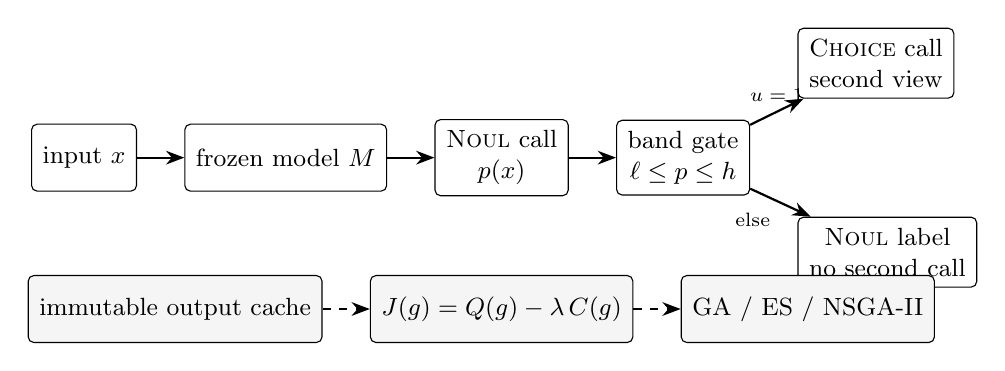
\begin{tikzpicture}[
  font=\small,
  >=Stealth,
  node distance=6mm,
  box/.style={draw, rounded corners=2pt, align=center, inner sep=4pt,
              minimum height=8.5mm, fill=white},
  arr/.style={->, thick},
  dashedarr/.style={->, thick, dashed}
]
\node[box] (x) {input $x$};
\node[box, right=of x] (m) {frozen model $M$};
\node[box, right=of m] (p) {\noul{} call\\$p(x)$};
\node[box, right=of p] (g) {band gate\\$\ell \le p \le h$};
\node[box, right=of g, yshift=12mm] (c) {\choice{} call\\second view};
\node[box, right=of g, yshift=-12mm] (n) {\noul{} label\\no second call};
\draw[arr] (x) -- (m);
\draw[arr] (m) -- (p);
\draw[arr] (p) -- (g);
\draw[arr] (g) -- node[above, font=\scriptsize]{$u=1$} (c);
\draw[arr] (g) -- node[below left, font=\scriptsize]{else} (n);
\node[box, below=10mm of p, fill=gray!8] (fit) {$J(g)=Q(g)-\lambda\,C(g)$};
\node[box, left=of fit, fill=gray!8] (cache) {immutable output cache};
\node[box, right=of fit, fill=gray!8] (search) {GA / ES / NSGA-II};
\draw[dashedarr] (cache) -- (fit);
\draw[dashedarr] (fit) -- (search);
\end{tikzpicture}
\caption{The routing setting. A frozen model answers a first \noul{} question;
a two-parameter gate decides whether the same model is asked a second
\choice{} question. Search operates entirely on cached outputs: a candidate
genome is scored by replaying the cache, and the optimiser only sees the scalar
fitness $J$. The dashed path is offline; the solid path is the deployed policy.}
\label{fig:pipeline}
\end{figure*}

For the binary tasks, CodeXGLUE and FinDVer, the first action is \noul{}: the
model answers a yes/no question and returns $p(x)=P(\text{true}\mid x)$. The
second action is \choice{}: the model selects between two named labels. In
CodeXGLUE the questions are whether a function contains a vulnerability and
whether it should be labelled \texttt{secure} or \texttt{vulnerable}; in
FinDVer they are whether a claim is supported and whether it should be labelled
\texttt{supported} or \texttt{not supported}. The cascade always pays for
\noul{} first and pays for \choice{} only when the gate opens. A policy is a
genome $g_{\mathrm{cas}}=(\ell,h,u)$ with $\ell,h\in[0,1]$ and
$u\in\{0,1\}$:
\begin{equation}
\pi_{g}(x)=
\begin{cases}
\choice(x), & u=1\!\land\!\ell\le p(x)\le h,\\
\noul(x), & \text{otherwise}.
\end{cases}
\label{eq:cascade}
\end{equation}
The gate uses the positive-class probability rather than symmetric confidence,
because a \noul{} question has a designated true label. Genome repair clips
$\ell$ and $h$ to $[0,1]$, swaps them when $\ell>h$, and maps $u$ to $\{0,1\}$.
Two fixed policies are special cases: $u=0$ is \noul-only, and
$u=1,\ell=0,h=1$ is fixed switch-only, which still pays for the first \noul{}
call and therefore costs two calls per row.

ProcessBench has a different action space. The model returns a ranked list of
candidate steps, and the policy decides whether to answer with the top-1 step or
to abstain. A genome $g_{\mathrm{abs}}=(t,v,m)$ with $t,m\in[0,1]$ and
$v\in\{0,1\}$ uses the top-1 probability $s_1(x)$ and the top-1/top-2 margin
$\Delta(x)$:
\begin{equation}
\mathrm{abstain}(x)=
\begin{cases}
\text{true}, & s_1(x)<t,\\
\text{true}, & v=1\,\land\,\Delta(x)<m,\\
\text{false}, & \text{otherwise}.
\end{cases}
\label{eq:abstain}
\end{equation}
When the required confidence fields are missing, the evaluator fails closed:
the row is forced to answer and is counted as incorrect rather than silently
dropped. We report coverage (the fraction of rows answered) and selective
accuracy (accuracy on answered rows).

Fitness combines task quality with the cost of the second call:
\begin{equation}
J(g)=Q(g)-\lambda\,C(g),
\label{eq:fitness}
\end{equation}
where $Q$ is macro-F1 on the binary tasks and step accuracy on ProcessBench,
$C(g)$ is the mean number of model calls per row minus one, and $\lambda=0.05$
is fixed before search. Macro-F1 is primary because both binary datasets are
class-imbalanced; accuracy is reported alongside it. The first \noul{} call is
charged to every policy, including \noul-only, so the cost term isolates the
incremental call rather than the total inference bill. Model outputs are
generated once and replayed from an immutable JSON cache, which makes candidate
evaluation deterministic and cheap.

The GA uses tournament selection, uniform crossover, Gaussian mutation and bit
flips on $u$. The ES is a $(\mu+\lambda)$ strategy that mutates the two
endpoints and fixes $u=1$. NSGA-II maintains a non-dominated front, optimising
accuracy and negative call cost on the binary tasks and selective accuracy and
coverage on ProcessBench; because its quality objective is accuracy rather than
macro-F1, we keep its intervals separate. The main budget is 24 unique genome
evaluations with seeds 17, 23 and 41; a five-seed extension adds 59 and 73. A
probe raises the CodeXGLUE/Vela budget to 48. Random search uses the same budget
and cache.

One property of the policy class shapes the calibration experiment. The gate
depends on $p(x)$ only through the interval $\ell\le p\le h$. Any strictly
monotone transformation of $p$---temperature scaling, for example---maps the
interval to another interval and induces the same set of switched rows up to a
reparameterisation of the endpoints. A monotone recalibration therefore cannot
change the best achievable band policy on a fixed pool. It can move rows between
bands, but it cannot create a distinction between repairable and harmful rows
that the raw ordering did not already contain. Calibration and routing are
therefore evaluated separately.

\section{Experimental Design}

The experiments use three tasks whose labels and group structure are fixed
before any policy is searched. CodeXGLUE defect detection provides 21{,}854
training, 2{,}732 dev and 2{,}732 test functions; the controller pools are drawn
only from the official training split, and functions are grouped by an exact
hash of their text so that identical functions cannot cross the internal
\texttt{search\_train}, \texttt{selection\_dev} and \texttt{confirm} pools
\citep{lu2021codexglue,zhou2019devign}. Each internal pool contains 60
functions. This controls duplicate-function leakage. FinDVer provides financial claims with \texttt{supported}/\texttt{not
supported} labels; its pools are grouped by report, and contain 60, 59 and 44
claims \citep{zhao2024findver}. The official FinDVer test labels are not used
for controller search. ProcessBench contains 3{,}400 annotated records over
2{,}842 mathematical problems; its pools are grouped by problem and contain 60
records each \citep{zheng2025processbench,cobbe2021gsm8k,lightman2024verify,uesato2022process}.
FinDVer internal pools are carved from official testmini and grouped by report
(41/16/16 groups; 60/59/44 claims); labels are used inside these pools for
fitting, thresholding and frozen evaluation. The official test split is
separate and read only by the locked-test evaluator. State is a \texttt{Claim:}
line, a blank line, then an \texttt{Evidence:} block. CodeXGLUE state is raw
function text
(positive rates 0.50/0.40/0.45). ProcessBench asks ``Which step contains the
earliest error?''; its state is the problem plus \texttt{[k] step} lines and an
\texttt{ALL STEPS CORRECT} sentinel.

All inference runs on one Windows machine with CPU-only PyTorch in FP32, two
threads and one model resident at a time. Laya is pinned to source revision
\texttt{b9fe351} and checkpoint revision \texttt{7b928d8}; Vela is pinned to
revision \texttt{d6f03aa}. Peak resident memory stays below 2.2~GB. The native
single-action baselines on \texttt{search\_dev} are as follows: CodeXGLUE
accuracy is 0.450/0.650 for Laya
(\noul/\choice) and 0.633/0.667 for Vela; FinDVer is 0.712/0.644 for Laya and
0.458/0.458 for Vela; ProcessBench \choice{} accuracy is 0.10 for both models.
The near-identical per-call latency of the two representations (about
2.2--2.8~s) is why call count, rather than a model-specific latency model, is
the cost term in Equation~\ref{eq:fitness}. The native numbers already contain a warning: the better representation depends
on the task and the model, and on FinDVer the two Vela actions are
indistinguishable at the aggregate level.

The first experiment measures action complementarity without training a router. For each
task--model cell we take the better fixed action on \texttt{search\_train} and
freeze that direction; we then count rows where the alternative action repairs a
base error, rows where it breaks a correct base answer, and their difference.
The oracle headroom is the accuracy of a per-row oracle minus the accuracy of
the better fixed action. Because the direction is fixed on train, the held-out
net-repair numbers are not selected on the evaluation pool. We report net repair
in percentage points with a group-level percentile bootstrap (5{,}000
resamples), and pair it with the macro-F1 difference between fixed \choice{} and
fixed \noul{} on the same rows. ProcessBench has only one evaluated
representation, so its headroom is zero by construction and it is excluded from
the binary complementarity table.

The second experiment asks whether the signed incremental value of the second
action is predictable before that action is executed. The target is
$\Delta_i=\mathbf{1}[\choice_i\text{ correct}]-
\mathbf{1}[\noul_i\text{ correct}]\in\{-1,0,+1\}$. The features are deployable at the
moment of decision: $p$, $|p-0.5|$ and the binary entropy $-p\log p -
(1-p)\log(1-p)$; no \choice{} output, gold label or downstream feature is used.
We compare logistic regression, a shallow decision tree, a single confidence
threshold and a never-switch majority baseline. Training uses group-aware
three-fold out-of-fold predictions; the predictor and threshold are then chosen
together on \texttt{selection\_dev} by cost-adjusted net utility, frozen, and
evaluated once on \texttt{confirm}. Net utility is (repairs $-$ regressions)
divided by the number of rows; the cost-adjusted variant subtracts
$\lambda=0.05$ per switch. A champion that switches every row is retained, because it reveals
whether the predictor adds anything beyond fixed switching.

The search comparison runs optimisers under a matched evaluation budget. GA, ES and NSGA-II
are run on the cached pools with 24 unique genome evaluations and seeds 17, 23
and 41; the five-seed extension adds 59 and 73. Random search receives the same
budget. The primary deployment comparison is pre-specified: the GA genome
selected on \texttt{search\_train} is frozen and compared with fixed
switch-only on \texttt{confirm} using paired group-bootstrap macro-F1 intervals.
All other cell-level comparisons are exploratory and are reported with effect
estimates and intervals rather than as significance claims. We then examine the
search trajectory itself: best-so-far fitness per generation, the number of
unique genomes actually evaluated, the fraction of single-gene mutations that
leave fitness unchanged, the rank correlation between train and dev fitness
across the archive, and the effect of raising the budget cap from 24 to 48 on
CodeXGLUE with Vela.

Two boundary checks test whether the conclusions generalise. The transfer experiment freezes each source-task
genome and applies it to every target task and pool without re-searching;
diagonal cells are same-task deployment checks, off-diagonal cells are true
transfer. The fault map partitions rows by task, model and a confidence band
derived from \noul{} probability or candidate margin, and reports the error
severity of each cell on discover, dev and confirm. A cell is eligible when it
contains at least eight rows on the discover pool, and it is confirmed when the
dev or confirm severity is within 0.15 of the discover severity.

Two statistical details matter for reading the tables. All binary comparisons
use paired group bootstrap with 5{,}000 resamples and a fixed random state
\citep{efron1993bootstrap}; the resampling unit is the group (function hash or
report), not the row, so dependence within a report is preserved. We report
McNemar exact tests for repair/harmful counts \citep{mcnemar1947} and Wilson
intervals for within-cell severity \citep{wilson1927}, but we do not call a
result significant on the basis of a single seed or a single pool. The locked
test was run once under a protocol frozen before any test call. The confirm
pools are held out from search and threshold selection but have been inspected
during analysis.

\section{Results and Discussion}
\label{sec:results}

The first question is whether the action set offers anything to route. Table
\ref{tab:complementarity} and Figure~\ref{fig:headroom}
(Appendix~\ref{app:extra}) answer it at the level of individual rows. Gross
complementarity is not scarce. On CodeXGLUE with Laya, \choice{} repairs 14 of
the 60 \noul{} errors, and the per-row oracle reaches 0.783 accuracy against
0.550 for the better fixed action, a headroom of 0.233. The same cell shows why
headroom is a poor promise: \choice{} breaks 15 correct \noul{} answers, so the
net count on the training pool is $-1$ and the net-repair interval spans zero.
The other three binary cells have smaller gross opportunities (headroom
0.067--0.100) and net counts between $-6$ and $+1$. Across the four cells, the
training pool never produces a net repair distinguishable from zero.

Held-out pools do not turn the gross opportunity into a stable net gain. The
CodeXGLUE/Laya cell gains 20.0 points on \texttt{selection\_dev}
($[+1.7,+38.3]$), but the same frozen direction gains only 1.7 points on confirm
($[-18.3,+20.0]$). That gap is a selection-pool effect, not a routing effect:
dev is the pool on which the direction was chosen. FinDVer with Laya is the
exception that tests the narrative. Its confirm net repair is $+13.6$ points
$[+2.0,+24.6]$, and the fixed-action accuracy difference is $+0.136$
$[+0.020,+0.246]$. The corresponding macro-F1 difference, however, is $+0.111$
with an interval that crosses zero, and the better fixed action reverses from
\noul{} on dev to \choice{} on confirm. The cell therefore contains a real
accuracy-level repair signal on confirm, but not a macro-F1 gain, and not a
direction that a train-selected policy could have known to exploit. CodeXGLUE
with Vela moves the other way: the frozen direction is \choice{}-to-\noul{},
the train net is $-6$, and confirm is exactly zero. FinDVer with Vela is negative
on confirm ($-2.3$ points). Complementarity exists in the action set, but it is
sparse, metric-dependent and pool-dependent.

\begin{table*}[t]
\centering
\footnotesize
\caption{Action complementarity with the train-selected direction frozen across
pools ($n=60$ per training cell; FinDVer dev/confirm: 59/44). \emph{Headroom} is the accuracy gain of a per-row
oracle over the better fixed action on \texttt{search\_train};
\emph{repair/harmful} counts rows where the alternative fixes or breaks the
base decision. Net repair is the paired difference in percentage points
(alternative minus base) with a 95\% group-bootstrap interval on dev and
confirm. Headroom is an upper bound, not a deployable gain.}
\label{tab:complementarity}
\begin{tabular}{@{}llrrrr@{}}
\toprule
Task / model & Direction & Headroom & Repair/harmful & Net dev (95\% CI) & Net confirm (95\% CI) \\
\midrule
CodeXGLUE / Laya & Noul$\to$Choice & 0.233 & 14/15 & +20.0 [+1.7, +38.3] & +1.7 [-18.3, +20.0] \\
CodeXGLUE / Vela & Choice$\to$Noul & 0.067 & 4/10 & -3.3 [-15.0, +8.3] & +0.0 [-15.0, +15.0] \\
FinDVer / Laya & Noul$\to$Choice & 0.083 & 5/6 & -6.8 [-23.3, +6.0] & +13.6 [+2.0, +24.6] \\
FinDVer / Vela & Choice$\to$Noul & 0.100 & 6/7 & +0.0 [-9.1, +11.5] & -2.3 [-10.3, +5.0] \\
\bottomrule
\end{tabular}
\end{table*}


The location of the repairs matters as much as their count. Figure
\ref{fig:repair} (Appendix~\ref{app:extra}) plots the repair rate against the
\noul{} probability bin. Repairs concentrate in the middle and high bands,
around $p\in[0.4,0.8]$, and are close to zero in the lowest band. This is the
opposite of what a confidence cascade assumes: a threshold rule switches when
the model is uncertain, which is precisely where \choice{} is least likely to
fix anything, because the rows it can repair are rows where \noul{} was
confident and wrong. It also explains why calibration cannot rescue the router:
recalibration moves probability mass monotonically, but it does not move
repairable rows from the middle of the distribution to the low-confidence tail.

The second question is whether the incremental value of \choice{} is
predictable from the first call. Table~\ref{tab:predictability} reports
out-of-fold ranking quality and the net utility of the frozen dev-selected
policy. Ranking quality varies widely. Logistic regression reaches 0.674 on
CodeXGLUE with Laya and 0.919 on FinDVer with Vela; the tree reaches 0.739 on
CodeXGLUE with Laya. On FinDVer with Laya both predictors are near chance (0.455
and 0.466), unsurprising given that the cell has only five training repairs. The
policy results are weaker than the ranking results. The best dev policy for
CodeXGLUE with Laya is logistic regression with a threshold that switches every
row: dev net $+20.0$ points, confirm net $+1.7$ points and a cost-adjusted
$-3.3$. The FinDVer/Vela cell, despite the highest OOF AUROC, chooses a policy
with dev net $+3.4$ and confirm net $-2.3$ (zero repairs, one regression).
FinDVer with Laya selects a tree that switches one row and gains 2.3 points on
confirm, a point estimate built on a single decision. CodeXGLUE with Vela is
positive on dev ($+3.3$) and negative on confirm ($-1.7$). In no cell does a
high ranking score translate into a confirm net utility that is both positive
and estimated with enough support to matter.

\begin{table*}[t]
\centering
\scriptsize
\caption{Signed incremental-utility prediction. Target
$\Delta_i=\mathbf{1}[\textsc{Choice}_i\text{ correct}]-
\mathbf{1}[\textsc{Noul}_i\text{ correct}]\in\{-1,0,+1\}$. OOF $\rho$ is the
Spearman correlation under group-aware three-fold CV on \texttt{search\_train};
the threshold is selected on \texttt{search\_dev} and frozen for
\texttt{confirm}. Net utility is mean $\Delta$ minus $\lambda=0.05$ per switch,
in points, with a 95\% group-bootstrap interval; the last column is
switches/rows.}
\label{tab:predictability}
\begin{tabular}{@{}lrrrrrr@{}}
\toprule
Task / model & OOF $\rho$ & AUROC repair & AUROC reg. & Dev net & Confirm net (95\% CI) & Switches \\
\midrule
CodeXGLUE / Laya & -0.02 & 0.360 & 0.607 & +21.7 & +0.0 [-18.8, +13.0] & 42/60 \\
CodeXGLUE / Vela & +0.19 & 0.744 & 0.335 & +3.3 & -1.7 [-19.8, +8.5] & 54/60 \\
FinDVer / Laya & +0.13 & 0.458 & 0.707 & +1.7 & +0.0 [-0.3, +0.0] & 1/44 \\
FinDVer / Vela & -0.17 & 0.396 & 0.361 & +3.4 & -2.3 [-7.7, -0.1] & 5/44 \\
\bottomrule
\end{tabular}
\end{table*}


Calibration is the most natural explanation for a failed probability-based
router, so it serves as a control. Table~\ref{tab:calibration} and
Figure~\ref{fig:calibration} in Appendix~\ref{app:extra} show that raw
probabilities are poorly calibrated on confirm: ECE ranges from 0.090 to 0.290
and Brier scores from 0.218 to 0.287. Temperature scaling, fitted on
\texttt{search\_train}, reduces ECE in three of four cells (to 0.045--0.169) and
Brier in all four. Routing is unaffected: raw probabilities give confirm net
repairs of $-5.0$, $0.0$, $+2.3$ and $-2.3$ points, temperature-scaled ones give
$-1.7$, $+1.7$, $0.0$ and $0.0$, as the invariance argument in
Section~\ref{sec:method} predicts. The repair AUROC makes the point directly:
0.791, 0.444, 0.336 and 0.095 for the four cells; in the last two the
probability ranks repairable rows \emph{below} chance. A calibrated probability
of the current answer is not a calibrated probability of the alternative
action's value.

The third question is whether search converts the available signal into a
deployable policy. Table~\ref{tab:search} summarises the comparison. GA versus
random search is the cleanest test of optimiser value: with five seeds, four
task--model cells and three pools, there are 60 paired macro-F1 comparisons, and
none has an interval that excludes zero. GA versus fixed switch-only has five
significant positive cells, all on the FinDVer/Vela training pool and all with
an effect near $+0.12$; on dev and confirm, none of the 40 comparisons is
significant. The pre-registered deployment comparison---train-selected GA
against fixed switch-only on confirm---is null in every seed-level cell. ES
versus random search is null in all 30 comparisons; ES versus fixed switching
has three significant training cells and one significant confirm cell
(CodeXGLUE/Laya, seed 17, $+0.176$), the only confirm-level positive result, and
it is not replicated across seeds. NSGA-II deployment is significantly worse
than the fixed baseline in five dev cells and one confirm cell, with no positive
cell. The search problem has no stable held-out signal for any optimiser to
find.

\begin{table}[!b]
\centering
\small
\caption{Search comparisons under the pre-specified protocol. Counts are
paired group-bootstrap 95\% intervals that exclude zero; ``positive'' means the
evolved policy beats the stated baseline. GA and ES rows use macro-F1 on all
three pools with five seeds; the NSGA-II row uses accuracy on 12 dev and 12
confirm cells.}
\label{tab:search}
\begin{tabular}{@{}lrrl@{}}
\toprule
Comparison & Pos. & Neg. & Reading \\
\midrule
GA vs.\ random & 0 & 0 & no advantage (60) \\
GA vs.\ fixed & 5 & 0 & train-only (60) \\
ES vs.\ random & 0 & 0 & no advantage (30) \\
ES vs.\ fixed & 4 & 0 & one confirm (30) \\
NSGA-II vs.\ fixed & 0 & 6 & 5 dev, 1 confirm \\
\bottomrule
\end{tabular}
\end{table}


The trajectory diagnostics explain why more search does not help. In 15 of 21
logged GA/ES runs, best-so-far fitness does not improve after generation zero.
The neutral-mutation rate is 0.68--0.73, so most mutations produce a candidate
with exactly the same training score. The train--dev rank correlation is $-0.56$
and $-0.51$ for the two CodeXGLUE cells, meaning that candidates which look
better on train tend to look worse on dev, and $+0.44$ and $+0.99$ for the
FinDVer cells. Raising the budget from 24 to 48 on CodeXGLUE with Vela does not
close the gap: the GA evaluates only 22, 17 and 23 unique genomes under a cap of
48, while random search uses all 48. The search is not merely under-tuned; it is
under-informed.

The boundary checks ask whether these conclusions are artefacts of one pool or
task. Appendix~\ref{app:boundary} reports the transfer table and fault map.
Transfer is uniformly unhelpful: of 32 source--target by split units, six have a
significant paired difference against the target's fixed switch policy, and all
six are negative (two diagonal, four off-diagonal). The fault map is more
nuanced: of 15 eligible cells, 13 are confirmed on dev and 10 on confirm. The
highest confirm severities are on ProcessBench (Vela/mid 0.833, Laya/mid 0.875,
Vela/low 0.936, Laya/high 0.895). The mid-confidence cells are not simply the
low-confidence tail: a model can be moderately confident and still fail, and the
second representation fails on the same rows, so no gate on the first action's
probability can create a repair.

Taken together, the three questions describe a routing problem that fails before
the optimiser is asked to solve it: RQ1 finds gross but no stable net
complementarity, RQ2 finds ranking signal without reliable policy value, and RQ3
finds no held-out advantage because the landscape is flat and the training
ranking does not predict the dev ranking where it matters. Calibration improves
a different quantity: a model can report better probabilities for the question
it answered and still have nothing to say about whether a different question
would be answered better.

The practical implication is a change in the order of work. Before building a
router, measure whether the action set has net complementarity on held-out
groups and whether the candidate features rank repairable rows above chance. If
either check fails, a stronger optimiser will not help; if both pass, the
optimiser comparison can be run under a matched budget with a pre-registered
confirm comparison.

\section{Conclusion}

A probability returned with every typed judgment should decide when a second
judgment is worth buying. Our experiments on frozen Laya and Vela across three
tasks do not support that promise: evolutionary search produces no held-out
advantage over fixed policies or budget-matched random search.

Gross complementarity is real---a per-row oracle gains up to 23.3 accuracy
points---but harmful switches offset repairs, and the net balance is small,
metric-dependent and unstable across pools. Calibration and action-value
prediction dissociate: temperature scaling
improves ECE and Brier but not row order, and in both FinDVer cells the
probability ranks repairable rows below chance. The search landscape is flat:
most mutations are neutral, most runs plateau at generation zero, and the
training ranking does not predict the dev ranking.

Limits are part of the result: pools are small, the \noul{} template was not
audited, only two open models were run, and the locked test remains unrun. Next:
a supervision target judged by held-out net utility.

\bibliography{references}

\end{document}
